\documentclass[a4paper]{article}

%Russian-specific packages
%--------------------------------------
\usepackage[T2A]{fontenc}
\usepackage[utf8]{inputenc}
\usepackage[english, russian]{babel}
%for search in russian
\usepackage{cmap}
%--------------------------------------

%Math-specific packages
%--------------------------------------
\usepackage{amsmath}
\usepackage{amssymb}

%Format-specific packages
%--------------------------------------
\usepackage[left=1cm,
            right=1cm,
            top=1cm,
            bottom=1cm,
            bindingoffset=0cm]{geometry}
%--------------------------------------

% for theorems, lemmas and definitions
%--------------------------------------
\usepackage{amsthm}

\newtheorem{theorem}{Теорема}[section]

\theoremstyle{definition}
\newtheorem {definition}{Опр.}[section]
\newtheorem {task}{Задача}[section]

%--------------------------------------

%Roman enum items
\usepackage{enumerate}

% For graphics
%--------------------------------------
\usepackage{tikz}
\usetikzlibrary{
  % for faster compilation
  external
  % for cool arrows
  , arrows.meta
  % for angles
  , angles
  , quotes
  , babel
}
\tikzsetexternalprefix{tasks/}
\tikzexternalize

%--------------------------------------

% My commands
%--------------------------------------

\DeclareMathOperator{\sgn}{sgn}

\def\const{ \mathrm{const} }
\def\eps{ \varepsilon }
\def\Eps{ \mathcal{E} }

\def\R{ \mathbb{R} }
\def\Z{ \mathbb{Z} }
\def\C{ \mathbb{C} }
\def\E{ \mathrm{E} }
\def\D{ \mathrm{D} }
\def\P{ \mathrm{P} }

\def\littleO{ \overline{\overline{o}} }
\def\bigO{ \underline{\underline{\mathcal{O}}} }

\newcommand*{\norm}[1]{\left\lVert#1\right\rVert}
\newcommand*{\abs}[1]{\left\lvert#1\right\rvert}

% suppress page count
\pagestyle{empty}

\includeonly{
  tasks/task01/task,
  tasks/task02/task,
  tasks/task03/task,
  tasks/task04/task,
  tasks/task05/task,
  tasks/task06/task,
  tasks/task07/task,
  tasks/task08/task,
  tasks/task09/task,
  tasks/task10/task,
  tasks/task11/task,
  tasks/task12/task,
  tasks/task13/task,
  tasks/task14/task,
  tasks/task15/task,
  tasks/task16/task,
  tasks/task17/task,
  tasks/task18/task,
  tasks/task19/task,
  tasks/task20/task,
  tasks/task21/task,
  tasks/task22/task,
  tasks/task23/task,
  tasks/task24/task,
  tasks/task25/task,
  tasks/task26/task,
  tasks/task27/task,
  tasks/task28/task
}

\begin{document}

\begin{task}
\textbf{Предварительный материал из лекции (Гармонический осциллятор):}\\
Рассмотрим задачу:
$$
\mathcal{L}(x):=\int_{0}^{T_{0}}\left(\dot{x}^{2}-x^{2}\right) d t \rightarrow \mathrm{inf}, \quad x(0)=x\left(T_{0}\right)=0
$$

Тогда $L_{\dot{x}}=2 \dot{x}, L_{x}=-2 x$; уравнение Эйлера имеет вид $-\frac{d}{d t}(2 \dot{x})-2 x=0$, т.e. $\ddot{x}+x=0$.

Заметим, что $\hat{x}=0$ является допустимой экстремалью. Выясним, является ли она точкой локального или глобального минимума. Для этого используем следующий прием.

Пусть $\omega \in C^{1}\left[0, T_{0}\right]$. Тогда $$\int_{0}^{T_{0}} \left(\dot{\omega} x^{2}+2 \omega x \dot{x} \right)d t=\int_{0}^{T_{0}} \frac{d}{d t}\left(\omega x^{2}\right) d t=\left.\omega x^{2}\right|_{0} ^{T_{0}}=0\, \text{, если } x \in C_{0,0}^{1}\left[0, T_{0}\right].$$ \\
Значит, можно добавить этот ноль к интегралу:
$$
\int_{0}^{T_{0}}\left(\dot{x}^{2}-x^{2}\right) d t=\int_{0}^{T_{0}}\left(\dot{x}^{2}-x^{2}-\dot{\omega} x^{2}-2 \omega x \dot{x}\right) d t
$$

Подберем $\omega$ так, чтобы $\dot{x}^{2}-x^{2}-\dot{\omega} x^{2}-2 \omega x \dot{x}$ было полным квадратом: $\dot{x}^{2}-x^{2}-\dot{\omega} x^{2}-2 \omega x \dot{x}=(\dot{x}-\omega x)^{2}$, т.е. $-1-\dot{\omega}=\omega^{2}$. (Тогда $\int_{0}^{T_{0}}\left(\dot{x}^{2}-x^{2}\right) d t=$ $\left.\int_{0}^{T_{0}}(\dot{x}-\omega x)^{2} d t \geq 0.\right)$ Получаем, что $\omega=\operatorname{ctg}\left(t-t_{*}\right)$.
\\
\textbf{Задача}\\

1) Пусть $T_{0}>\pi,\ x(t)=c \sin \frac{\pi t}{T_{0}}$. Показать, что $\mathcal{L}(x)<0$ при $c \neq 0$. Почему проведенные выше рассуждения не проходят при $T_{0}>\pi$ и проходят при $T_{0}<\pi$ ?\\
2) Показать, что $\int_{0}^{\pi}\left(\dot{x}^{2}-x^{2}\right) d t=\int_{0}^{\pi}(\dot{x}-x \cdot \operatorname{ctg} t)^{2} d t \geqslant 0$.

\textbf{Решение.} 1) Вычисляем:
$$
\begin{gathered}
\int_{0}^{T_{0}}\left(\dot{x}^{2}-x^{2}\right) d t=c^{2} \int_{0}^{T_{0}}\left(\frac{\pi^{2}}{T_{0}} \cos ^{2} \frac{\pi t}{T_{0}}-\sin ^{2} \frac{\pi t}{T_{0}}\right) d t= \\
=\frac{c^{2}}{2}\left(\frac{\pi^{2}}{T_{0}^{2}} \int_{0}^{T_{0}}\left(1+\cos \frac{2 \pi t}{T_{0}}\right) d t-\int_{0}^{T_{0}}\left(1-\cos \frac{2 \pi t}{T_{0}}\right) d t\right)=\frac{c^{2} T_{0}}{2}\left(\frac{\pi^{2}}{T_{0}^{2}}-1\right)<0 .
\end{gathered}
$$

Напомним, что мы подбирали гладкую функцию $\omega$ так, чтобы

$$
\int_{0}^{T_{0}}\left(\dot{x}^{2}-x^{2}\right) d t=\int_{0}^{T_{0}}(\dot{x}-\omega x)^{2} d t
$$

при этом $\omega$ была решением дифференциального уравнения $\dot{\omega}=-1-\omega^{2}$. Значит, $\omega(t)=$ $\operatorname{ctg}(t-a)$.

Если $T_{0}<\pi$, то можно подобрать $a$ (в данном случае подойдет $a = 0$) так, чтобы $\operatorname{ctg}(t-a)$ была гладкой на $\left[0, T_{0}\right]$. Если $T_{0}>\pi$, то для любого $a$ функция $\omega$ будет иметь точку разрыва в интервале $\left(0, T_{0}\right)$, т.к. $ctg$ гладко определен на $(\pi n ,\ \pi n + \pi)$ и имеет разрывы в точках $\pi n$.

2) Преобразуем правую часть условия:
$$
\begin{gathered}
0 \leq\int_{0}^{\pi}(\dot{x}-x \cdot \operatorname{ctg} t)^{2} d t=\int_{0}^{\pi}\left(\dot{x}^{2}-2 x \dot{x} \operatorname{ctg} t+x^{2} \operatorname{ctg}^{2} t\right) d t= 
\end{gathered}
$$\\
интегрируем среднее слагаемое по частям и используем $\dot{ctg}+ctg^{2}=-1$:
$$
\begin{gathered}
=\int_{0}^{\pi}\left(\dot{x}^{2}+x^{2}(\operatorname{ctg} t)^{\prime}+x^{2} \operatorname{ctg}^{2} t\right) d t+\left.x^{2}(t) \operatorname{ctg} t\right|_{0} ^{\pi}=\int_{0}^{\pi}\left(\dot{x}^{2}-x^{2}\right) d t+\left.x^{2}(t) \operatorname{ctg} t\right|_{0} ^{\pi} .
\end{gathered}
$$

Так как $x \in C^{1}[0, \pi]$ и $x(0)=0$, то $x(t)=O(t)$ в окрестности нуля; так как $\operatorname{ctg} t=O(1 / t)$ в окрестности нуля, то $x^{2}(t) \operatorname{ctg} t=O(t) \underset{t \rightarrow 0}{\rightarrow} 0$. Аналогично $x^{2}(t) \operatorname{ctg} t=O(\pi-t) \underset{t \rightarrow \pi}{\rightarrow} 0$. Значит, $\left.x^{2}(t) \operatorname{ctg} t\right|_{0} ^{\pi}=0$ и равенство доказано.

\end{task}

\begin{task}
Привести пример функции $f: \mathbb{R} \rightarrow \mathbb{R}$, всюду дифференцируемой по Фреше, но не строго дифференцируемой в нуле.

\textbf{Доказательство:}
Рассмотрим функцию $f$:
\[
f(x)= \begin{cases}0, & x=0 \\ x^2 \sin \left(\frac{1}{x}\right), & x \neq 0\end{cases} 
\]

\begin{figure}[h!]
\centering
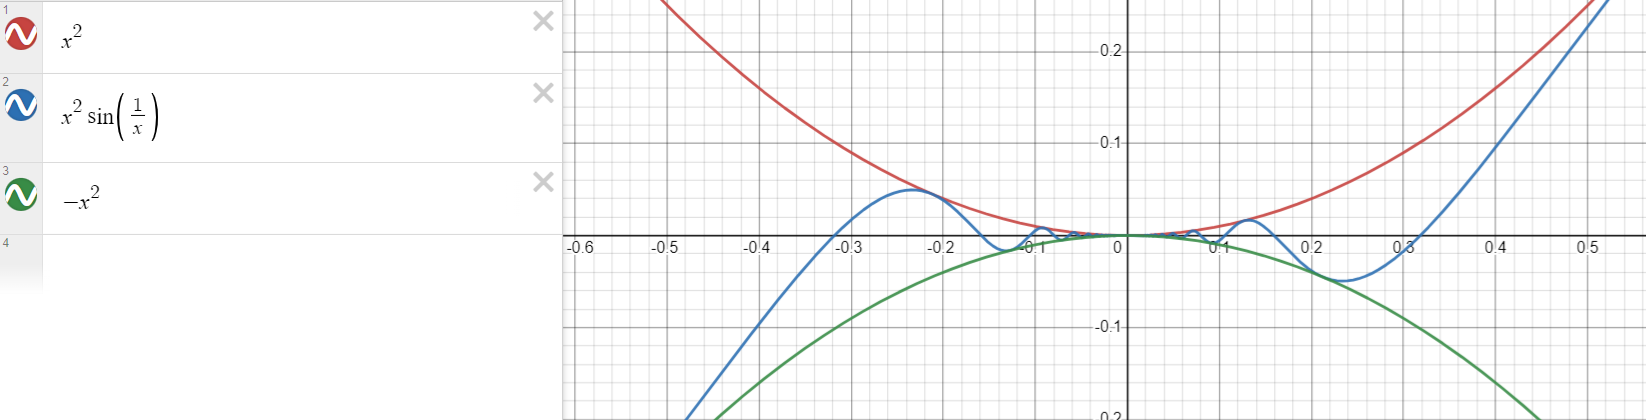
\includegraphics[width=0.99\linewidth]{tasks/task10/image.png}
\end{figure}
 
$f$ дифференцируема по Фреше в $x \neq 0$ (по правилу Лейбница):
\[\begin{aligned}
& {(x + h)}^{2} = x^2 +2xh+ \bar{o}(|h|)\\
& \sin{\frac{1}{x+h}} = \sin{\frac{1}{x}} + \frac{-1}{x^2} \cos{\frac{1}{x}}h + \bar{o}(|h|)
\end{aligned}\]
$|f(x)| \leq x^2 \implies f^{\prime}(0)=0$ и $f(x)-f(0)=f(x) =\bar{o}(|x|), |x| \rightarrow 0 $
то есть f диф. по Фреше в 0, тогда и на всем $\mathbb{R}$

Предположим противное: $f$ строго дифференцируемо в $0$.

По определению,  для любого $\varepsilon>0$ существует $\delta>0$ такое, что для любых $x_1, x_2 \in O_\delta\left(x_0\right)$ выполнено
\[\begin{aligned}
&|f\left(x_1\right)-f\left(x_2\right)-A\left(x_1-x_2\right)|\leq \varepsilon|x_1-x_2| \\
&f^{\prime}(0)=0 \implies |f\left(x_1\right)-f\left(x_2\right)|\leq \varepsilon|x_1-x_2|\leq 2\varepsilon \delta \\
& x\neq 0:  f^{\prime}(x)=2 x \sin \frac{1}{x}+x^2 \cos \frac{1}{x}\left(-1 \cdot \frac{1}{x^2}\right)=2 x \sin \left(\frac{1}{x}\right)-\cos \frac{1}{x} \nrightarrow 0, x \rightarrow 0 \\
& \text{потому что } \lim _{x \rightarrow 0} x \sin \frac{1}{x}=0 \text{ и } \lim _{x \rightarrow 0} \cos \frac{1}{x} \text{ не существует.} \\
& \text{Тогда }\exists \xi_n \rightarrow 0 \quad\left|f^{\prime}\left(\xi_n\right)\right| \geqslant c>0 \\
& f\left(\xi_n+h_n\right)-f\left(\xi_n\right)=f^{\prime}\left(\xi_n\right) h_n+\bar{o}\left(h_n\right) \text{ (по опр. диф. по Фреше)}\\
& h_n \longrightarrow 0 :\\
& \left|f\left(\xi_n+h_n\right)-f\left(\xi_n\right)\right| \geqslant C\left|h_n\right|
\end{aligned}\]
Получили противоречие. $f$ не является строго дифференцируемой в нуле.
\end{task}

\begin{task}
Привести пример функции $f: \mathbb{R} \rightarrow \mathbb{R}$, всюду дифференцируемой по Фреше, но не строго дифференцируемой в нуле.

\textbf{Доказательство:}
Рассмотрим функцию $f$:
\[
f(x)= \begin{cases}0, & x=0 \\ x^2 \sin \left(\frac{1}{x}\right), & x \neq 0\end{cases} 
\]

\begin{figure}[h!]
\centering
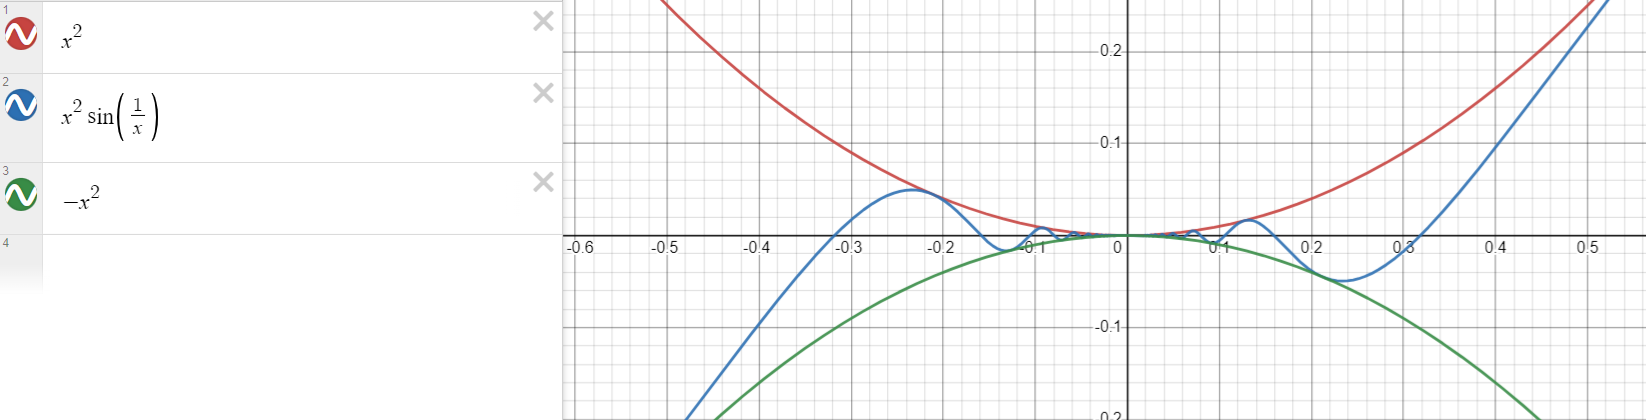
\includegraphics[width=0.99\linewidth]{tasks/task10/image.png}
\end{figure}
 
$f$ дифференцируема по Фреше в $x \neq 0$ (по правилу Лейбница):
\[\begin{aligned}
& {(x + h)}^{2} = x^2 +2xh+ \bar{o}(|h|)\\
& \sin{\frac{1}{x+h}} = \sin{\frac{1}{x}} + \frac{-1}{x^2} \cos{\frac{1}{x}}h + \bar{o}(|h|)
\end{aligned}\]
$|f(x)| \leq x^2 \implies f^{\prime}(0)=0$ и $f(x)-f(0)=f(x) =\bar{o}(|x|), |x| \rightarrow 0 $
то есть f диф. по Фреше в 0, тогда и на всем $\mathbb{R}$

Предположим противное: $f$ строго дифференцируемо в $0$.

По определению,  для любого $\varepsilon>0$ существует $\delta>0$ такое, что для любых $x_1, x_2 \in O_\delta\left(x_0\right)$ выполнено
\[\begin{aligned}
&|f\left(x_1\right)-f\left(x_2\right)-A\left(x_1-x_2\right)|\leq \varepsilon|x_1-x_2| \\
&f^{\prime}(0)=0 \implies |f\left(x_1\right)-f\left(x_2\right)|\leq \varepsilon|x_1-x_2|\leq 2\varepsilon \delta \\
& x\neq 0:  f^{\prime}(x)=2 x \sin \frac{1}{x}+x^2 \cos \frac{1}{x}\left(-1 \cdot \frac{1}{x^2}\right)=2 x \sin \left(\frac{1}{x}\right)-\cos \frac{1}{x} \nrightarrow 0, x \rightarrow 0 \\
& \text{потому что } \lim _{x \rightarrow 0} x \sin \frac{1}{x}=0 \text{ и } \lim _{x \rightarrow 0} \cos \frac{1}{x} \text{ не существует.} \\
& \text{Тогда }\exists \xi_n \rightarrow 0 \quad\left|f^{\prime}\left(\xi_n\right)\right| \geqslant c>0 \\
& f\left(\xi_n+h_n\right)-f\left(\xi_n\right)=f^{\prime}\left(\xi_n\right) h_n+\bar{o}\left(h_n\right) \text{ (по опр. диф. по Фреше)}\\
& h_n \longrightarrow 0 :\\
& \left|f\left(\xi_n+h_n\right)-f\left(\xi_n\right)\right| \geqslant C\left|h_n\right|
\end{aligned}\]
Получили противоречие. $f$ не является строго дифференцируемой в нуле.
\end{task}

\begin{task}
(задача о геодезических на плоскости Лобачевского.) Найти допустимые экстремали в задаче

$$
\int_{t_{0}}^{t_{1}} \frac{\sqrt{1+\dot{x}^{2}}}{x} d t \rightarrow \operatorname{extr}, x\left(t_{0}\right)=x_{0}, \quad x\left(t_{1}\right)=x_{1}, \quad x>0
$$

\textbf{Решение.} 
Имеем $L_{\dot{x}}=\frac{\dot{x}}{x \sqrt{1+\dot{x}^{2}}}, L_{\dot{x} \dot{x}}=\frac{1}{x\left(1+\dot{x}^{2}\right)^{3 / 2}}>0$. Значит, $\hat{x} \in$ $C^{2}\left[t_{0}, t_{1}\right]$ и $\dot{\hat{x}}(t) L_{\dot{x}}(\hat{x}(t), \dot{\hat{x}}(t))-L(\hat{x}(t), \dot{\hat{x}}(t))=$ const.

Проверим, что допустимая экстремаль не может обращаться в константу ни на каком невырожденном интервале. Это видно из уравнения Эйлера:

$$
-\frac{d}{d t} \frac{\dot{x}}{x \sqrt{1+\dot{x}^{2}}}-\frac{\sqrt{1+\dot{x}^{2}}}{x^{2}}=0
$$

(тогда бы получилось равенство $1 / \hat{x}^{2}(t) \equiv 0$ ).

Из уравнения $\dot{x} L_{\dot{x}}-L=$ const получаем

$$
\dot{x} \cdot \frac{\dot{x}}{x \sqrt{1+\dot{x}^{2}}}-\frac{\sqrt{1+\dot{x}^{2}}}{x}=\text { const. }
$$

Значит, $\frac{1}{x \sqrt{1+\dot{x}^{2}}}=$ const. Получаем $1+\dot{x}^{2}=\frac{c^{2}}{x^{2}}$, или $\dot{x}= \pm \sqrt{1-\frac{c^{2}}{x^{2}}}$. На промежутках, где $\dot{x} \neq 0$, решаем это дифференциальное уравнение и получаем

$$
t-a= \pm \int \frac{d x}{\sqrt{1-\frac{c^{2}}{x^{2}}}}= \pm \frac{1}{2} \int \frac{d x^{2}}{\sqrt{x^{2}-c^{2}}}= \pm \sqrt{x^{2}-c^{2}}
$$

Возводим в квадрат и получаем $x^{2}+(t-a)^{2}=c^{2}$. Это уравнение окружности с центром на горизонтальной оси.

Если в какой-то точке $\dot{x}$ обращается в 0 , то условия теоремы единственности нарушаются, но всё равно экстремаль задается уравнением окружности (склеивается из двух дуг окружностей; в силу гладкости обе дуги принадлежат одной и той же окружности; горизонтальных "вставок" быть не может, т.к. экстремаль не равна константе на интервалах).

Итак, геодезические - дуги окружности с центром на горизонтальной оси.

Утверждается, что найденная допустимая экстремаль будет точкой глобального минимума. В самом деле, $L_{\dot{x} \dot{x}}>0$ при $x>0$, так что $L$ выпукла по $\dot{x}$.

\end{task}
\begin{task}
Привести пример функции $f: \mathbb{R} \rightarrow \mathbb{R}$, всюду дифференцируемой по Фреше, но не строго дифференцируемой в нуле.

\textbf{Доказательство:}
Рассмотрим функцию $f$:
\[
f(x)= \begin{cases}0, & x=0 \\ x^2 \sin \left(\frac{1}{x}\right), & x \neq 0\end{cases} 
\]

\begin{figure}[h!]
\centering
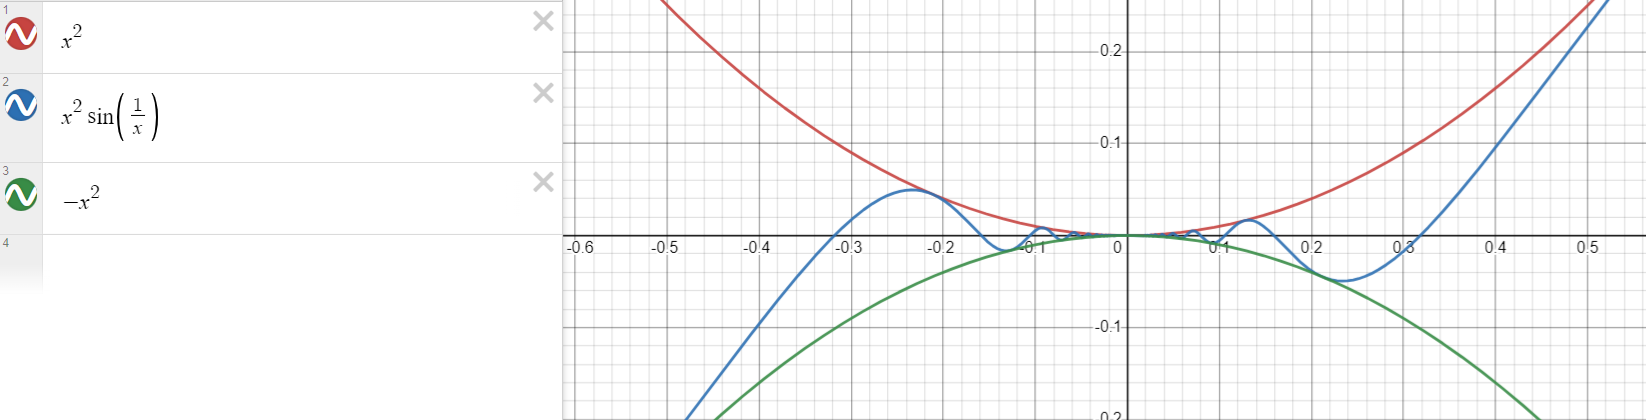
\includegraphics[width=0.99\linewidth]{tasks/task10/image.png}
\end{figure}
 
$f$ дифференцируема по Фреше в $x \neq 0$ (по правилу Лейбница):
\[\begin{aligned}
& {(x + h)}^{2} = x^2 +2xh+ \bar{o}(|h|)\\
& \sin{\frac{1}{x+h}} = \sin{\frac{1}{x}} + \frac{-1}{x^2} \cos{\frac{1}{x}}h + \bar{o}(|h|)
\end{aligned}\]
$|f(x)| \leq x^2 \implies f^{\prime}(0)=0$ и $f(x)-f(0)=f(x) =\bar{o}(|x|), |x| \rightarrow 0 $
то есть f диф. по Фреше в 0, тогда и на всем $\mathbb{R}$

Предположим противное: $f$ строго дифференцируемо в $0$.

По определению,  для любого $\varepsilon>0$ существует $\delta>0$ такое, что для любых $x_1, x_2 \in O_\delta\left(x_0\right)$ выполнено
\[\begin{aligned}
&|f\left(x_1\right)-f\left(x_2\right)-A\left(x_1-x_2\right)|\leq \varepsilon|x_1-x_2| \\
&f^{\prime}(0)=0 \implies |f\left(x_1\right)-f\left(x_2\right)|\leq \varepsilon|x_1-x_2|\leq 2\varepsilon \delta \\
& x\neq 0:  f^{\prime}(x)=2 x \sin \frac{1}{x}+x^2 \cos \frac{1}{x}\left(-1 \cdot \frac{1}{x^2}\right)=2 x \sin \left(\frac{1}{x}\right)-\cos \frac{1}{x} \nrightarrow 0, x \rightarrow 0 \\
& \text{потому что } \lim _{x \rightarrow 0} x \sin \frac{1}{x}=0 \text{ и } \lim _{x \rightarrow 0} \cos \frac{1}{x} \text{ не существует.} \\
& \text{Тогда }\exists \xi_n \rightarrow 0 \quad\left|f^{\prime}\left(\xi_n\right)\right| \geqslant c>0 \\
& f\left(\xi_n+h_n\right)-f\left(\xi_n\right)=f^{\prime}\left(\xi_n\right) h_n+\bar{o}\left(h_n\right) \text{ (по опр. диф. по Фреше)}\\
& h_n \longrightarrow 0 :\\
& \left|f\left(\xi_n+h_n\right)-f\left(\xi_n\right)\right| \geqslant C\left|h_n\right|
\end{aligned}\]
Получили противоречие. $f$ не является строго дифференцируемой в нуле.
\end{task}

\begin{task} \label{task6}
    Найти допустимые экстремали в задаче
    \[  \int_{-T_{0}}^{T_{0}} x\sqrt{1 + \dot{x}} \,dt \rightarrow extr\text{, }x(-T_{0}) = x(T_{0}) = \xi\text{, } x > 0 \]
    В зависимости от $\xi > 0$ установить, сколько может быть допустимых экстремалей. \\
    \textbf{Решение:} \\
    \[L_{\dot{x}} = \frac{x\dot{x}}{\sqrt{1 + \dot{x}^2}}\]
    \[L_{\dot{x}\dot{x}} = {\frac{x}{(1 + \dot{x}^{2})}^ {3/2}} > 0,\]
    Решение уравнения Эйлера $\hat{x} \in C^2[-T_{0}, T_{0}]$ и $\hat{x}(t)\dot{L_{x}}(\hat{x}(t),
        \dot{\hat{x}}(t)) - L(\hat{x}(t),
        \dot{\hat{x}}(t)) = const$.\\
    Проверим, что допустимая экстремаль не может обращаться в константу ни на каком невырожденном отрезке. Это видно из уравнения Эйлера:
    \[-\frac{d}{dt} \frac{x\dot{x}}{\sqrt{1 + \dot{x}^2}} + \sqrt{1 + \dot{x}} = 0\]
    Решений нет. \\
    Из уравнения $\dot{x}L_{\dot{x}} - L = const$ получаем: \\
    \[ \dot{x} \frac{x\dot{x}}{\sqrt{1 + \dot{x}^2}} - x\sqrt{1 + \dot{x}} = const\]
    \[\frac{x}{\sqrt{1 + \dot{x}^2}} = const = C \Rightarrow 1 + \dot{x}^2 = \frac{x^2}{C^2} \Rightarrow \dot{x} = \pm \sqrt{\frac{x^2}{C^2} - 1} \Rightarrow dt = \pm \frac{dx}{\sqrt{\frac{x^2}{C^2} - 1}}\]
    \[t + a = \pm \int_{}^{}\frac{1}{\sqrt{\frac{x^2}{C^2} - 1}} \,dx = \left| x = Cch(\tau) \right| = \pm \int_{}^{}\frac{C sh(\tau)}{|sh(\tau)|} \,d\tau \]
    \[t + a = \pm C\tau \Rightarrow \frac{t+a}{C} = \pm \tau \Rightarrow ch\left(\frac{t+a}{C}\right) = ch(\tau) = \frac{x}{C} \Rightarrow x = Cch\left(\frac{t+a}{C}\right)\]
    \[x(-T_{0}) = x(T_{0}) \Rightarrow x = Cch\left(\frac{t}{C}\right)\]
    $C$ --- решение уравнения $Cch\left(\frac{T_{0}}{C}\right) = \xi$. Пусть $b = \frac{1}{C}$, тогда $ch(T_{0}b) = \xi b$. $ch(T_{0}b)$ --- выпуклая вниз функция, а $\xi b$ --- линейная $\Rightarrow$ может быть 0, 1 или 2 решениия.
    \[\xi_{*} > 0 \text{ --- случай касания.}\]
    \[\xi > \xi_{*} \text{ --- два решения.}\]
    \[\xi < \xi_{*} \text{ --- нет решений.}\]
    $ch(T_{0}b) = \xi_{*}b$, $T_{0}sh(T_{0}b) = \xi_{*}$. Исключаем $\xi_{*}$.
    \[ch(T_{0}b) = T_{0}bsh(T_{0}b)\]
    Отсюда находим $b$, а потом $\xi_{*}$.
\end{task}
\begin{task}
    Пусть $F: \mathbb{R}^2 \rightarrow \mathbb{R}$ задано равенством $F\left(x_1, x_2\right)=\sqrt[3]{x_1^2 x_2}$. Показать, что $F$ имеет вариацию по Лагранжу, но не дифференцируемо по Гато в нуле. \textbf{2)} Пусть $X$ -- бесконечномерное нормированное пространство, $F: X \rightarrow \mathbb{R}$ - линейный неограниченный функционал. Показать, что $F$ имеет вариацию по Лагранжу в нуле, но не дифференцируемо по Гато.
    
    \textbf{Решение.} \textbf{1)} Пусть $h = \left( h_1, h_2 \right)$. Тогда $F\left(t h_1, t h_2\right)=\sqrt[3]{\left(t h_1\right)^2 t h_2}=t \sqrt[3]{h_1^2 h_2}$. Значит,
    $$
    \frac{F\left(t h_1, t h_2\right)-F(0,0)}{t}=\sqrt[3]{h_1^2 h_2}, \quad F^{\prime}(0,0)\left[\left(h_1, h_2\right)\right]=\sqrt[3]{h_1^2 h_2}
    $$ 
    легко видеть, что это отображение нелинейно.\\
    \textbf{2)} Если функционал $F$ линеен, то $F(t h)-F(0)=t F(h)$; значит, $F^{\prime}(0)[h]=F(h)$. Это отображение линейно, но разрывно.
    
    \end{task}
\begin{task}
Привести пример функции $f: \mathbb{R} \rightarrow \mathbb{R}$, всюду дифференцируемой по Фреше, но не строго дифференцируемой в нуле.

\textbf{Доказательство:}
Рассмотрим функцию $f$:
\[
f(x)= \begin{cases}0, & x=0 \\ x^2 \sin \left(\frac{1}{x}\right), & x \neq 0\end{cases} 
\]

\begin{figure}[h!]
\centering
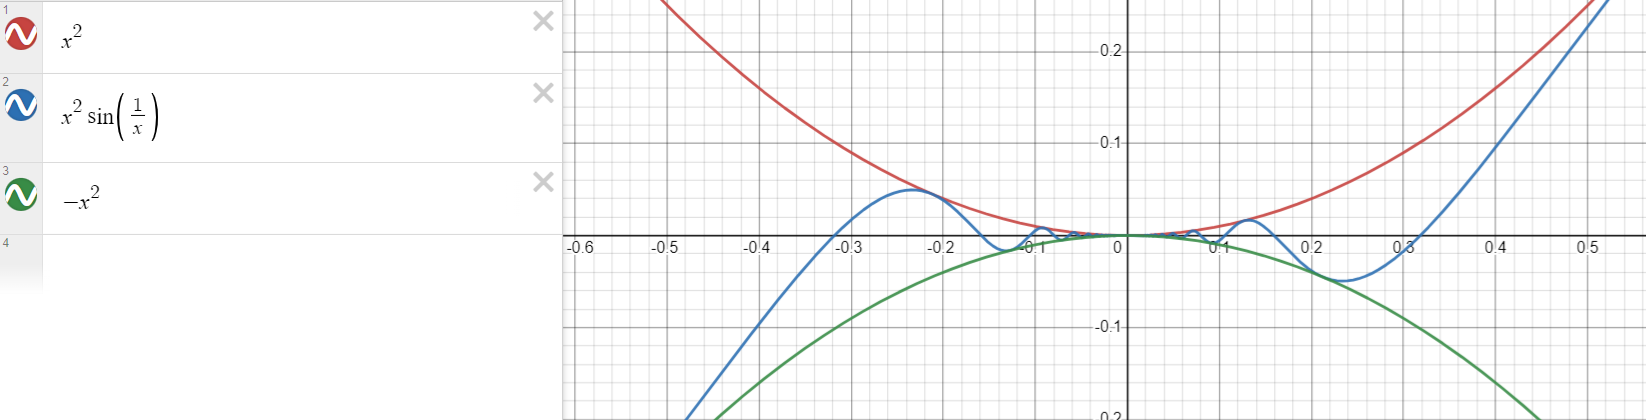
\includegraphics[width=0.99\linewidth]{tasks/task10/image.png}
\end{figure}
 
$f$ дифференцируема по Фреше в $x \neq 0$ (по правилу Лейбница):
\[\begin{aligned}
& {(x + h)}^{2} = x^2 +2xh+ \bar{o}(|h|)\\
& \sin{\frac{1}{x+h}} = \sin{\frac{1}{x}} + \frac{-1}{x^2} \cos{\frac{1}{x}}h + \bar{o}(|h|)
\end{aligned}\]
$|f(x)| \leq x^2 \implies f^{\prime}(0)=0$ и $f(x)-f(0)=f(x) =\bar{o}(|x|), |x| \rightarrow 0 $
то есть f диф. по Фреше в 0, тогда и на всем $\mathbb{R}$

Предположим противное: $f$ строго дифференцируемо в $0$.

По определению,  для любого $\varepsilon>0$ существует $\delta>0$ такое, что для любых $x_1, x_2 \in O_\delta\left(x_0\right)$ выполнено
\[\begin{aligned}
&|f\left(x_1\right)-f\left(x_2\right)-A\left(x_1-x_2\right)|\leq \varepsilon|x_1-x_2| \\
&f^{\prime}(0)=0 \implies |f\left(x_1\right)-f\left(x_2\right)|\leq \varepsilon|x_1-x_2|\leq 2\varepsilon \delta \\
& x\neq 0:  f^{\prime}(x)=2 x \sin \frac{1}{x}+x^2 \cos \frac{1}{x}\left(-1 \cdot \frac{1}{x^2}\right)=2 x \sin \left(\frac{1}{x}\right)-\cos \frac{1}{x} \nrightarrow 0, x \rightarrow 0 \\
& \text{потому что } \lim _{x \rightarrow 0} x \sin \frac{1}{x}=0 \text{ и } \lim _{x \rightarrow 0} \cos \frac{1}{x} \text{ не существует.} \\
& \text{Тогда }\exists \xi_n \rightarrow 0 \quad\left|f^{\prime}\left(\xi_n\right)\right| \geqslant c>0 \\
& f\left(\xi_n+h_n\right)-f\left(\xi_n\right)=f^{\prime}\left(\xi_n\right) h_n+\bar{o}\left(h_n\right) \text{ (по опр. диф. по Фреше)}\\
& h_n \longrightarrow 0 :\\
& \left|f\left(\xi_n+h_n\right)-f\left(\xi_n\right)\right| \geqslant C\left|h_n\right|
\end{aligned}\]
Получили противоречие. $f$ не является строго дифференцируемой в нуле.
\end{task}

\begin{task}
Привести пример функции $f: \mathbb{R} \rightarrow \mathbb{R}$, всюду дифференцируемой по Фреше, но не строго дифференцируемой в нуле.

\textbf{Доказательство:}
Рассмотрим функцию $f$:
\[
f(x)= \begin{cases}0, & x=0 \\ x^2 \sin \left(\frac{1}{x}\right), & x \neq 0\end{cases} 
\]

\begin{figure}[h!]
\centering
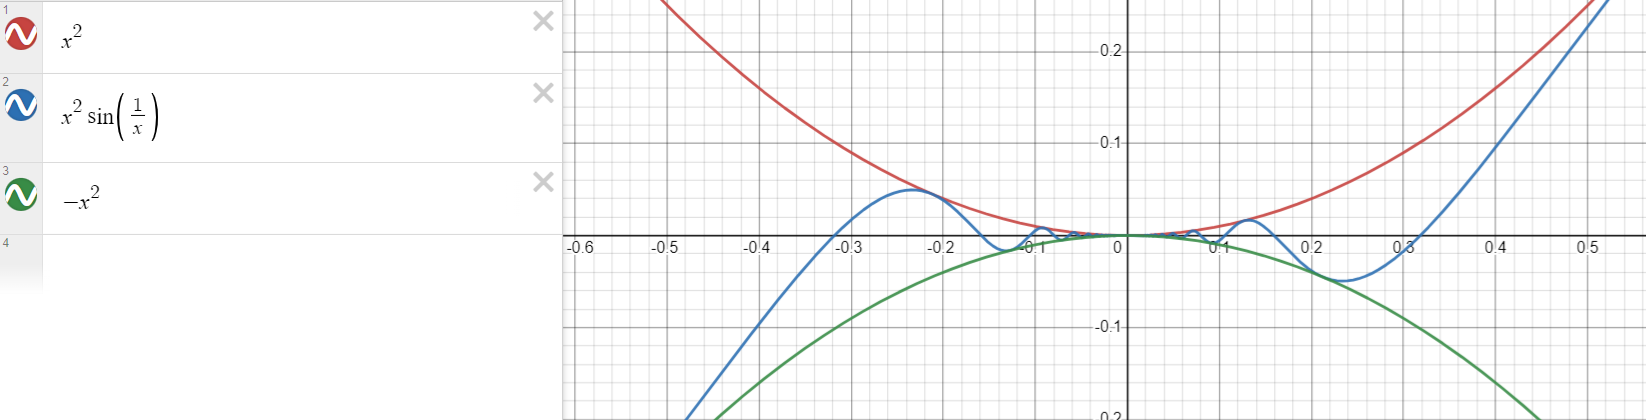
\includegraphics[width=0.99\linewidth]{tasks/task10/image.png}
\end{figure}
 
$f$ дифференцируема по Фреше в $x \neq 0$ (по правилу Лейбница):
\[\begin{aligned}
& {(x + h)}^{2} = x^2 +2xh+ \bar{o}(|h|)\\
& \sin{\frac{1}{x+h}} = \sin{\frac{1}{x}} + \frac{-1}{x^2} \cos{\frac{1}{x}}h + \bar{o}(|h|)
\end{aligned}\]
$|f(x)| \leq x^2 \implies f^{\prime}(0)=0$ и $f(x)-f(0)=f(x) =\bar{o}(|x|), |x| \rightarrow 0 $
то есть f диф. по Фреше в 0, тогда и на всем $\mathbb{R}$

Предположим противное: $f$ строго дифференцируемо в $0$.

По определению,  для любого $\varepsilon>0$ существует $\delta>0$ такое, что для любых $x_1, x_2 \in O_\delta\left(x_0\right)$ выполнено
\[\begin{aligned}
&|f\left(x_1\right)-f\left(x_2\right)-A\left(x_1-x_2\right)|\leq \varepsilon|x_1-x_2| \\
&f^{\prime}(0)=0 \implies |f\left(x_1\right)-f\left(x_2\right)|\leq \varepsilon|x_1-x_2|\leq 2\varepsilon \delta \\
& x\neq 0:  f^{\prime}(x)=2 x \sin \frac{1}{x}+x^2 \cos \frac{1}{x}\left(-1 \cdot \frac{1}{x^2}\right)=2 x \sin \left(\frac{1}{x}\right)-\cos \frac{1}{x} \nrightarrow 0, x \rightarrow 0 \\
& \text{потому что } \lim _{x \rightarrow 0} x \sin \frac{1}{x}=0 \text{ и } \lim _{x \rightarrow 0} \cos \frac{1}{x} \text{ не существует.} \\
& \text{Тогда }\exists \xi_n \rightarrow 0 \quad\left|f^{\prime}\left(\xi_n\right)\right| \geqslant c>0 \\
& f\left(\xi_n+h_n\right)-f\left(\xi_n\right)=f^{\prime}\left(\xi_n\right) h_n+\bar{o}\left(h_n\right) \text{ (по опр. диф. по Фреше)}\\
& h_n \longrightarrow 0 :\\
& \left|f\left(\xi_n+h_n\right)-f\left(\xi_n\right)\right| \geqslant C\left|h_n\right|
\end{aligned}\]
Получили противоречие. $f$ не является строго дифференцируемой в нуле.
\end{task}

\begin{task}
Привести пример функции $f: \mathbb{R} \rightarrow \mathbb{R}$, всюду дифференцируемой по Фреше, но не строго дифференцируемой в нуле.

\textbf{Доказательство:}
Рассмотрим функцию $f$:
\[
f(x)= \begin{cases}0, & x=0 \\ x^2 \sin \left(\frac{1}{x}\right), & x \neq 0\end{cases} 
\]

\begin{figure}[h!]
\centering
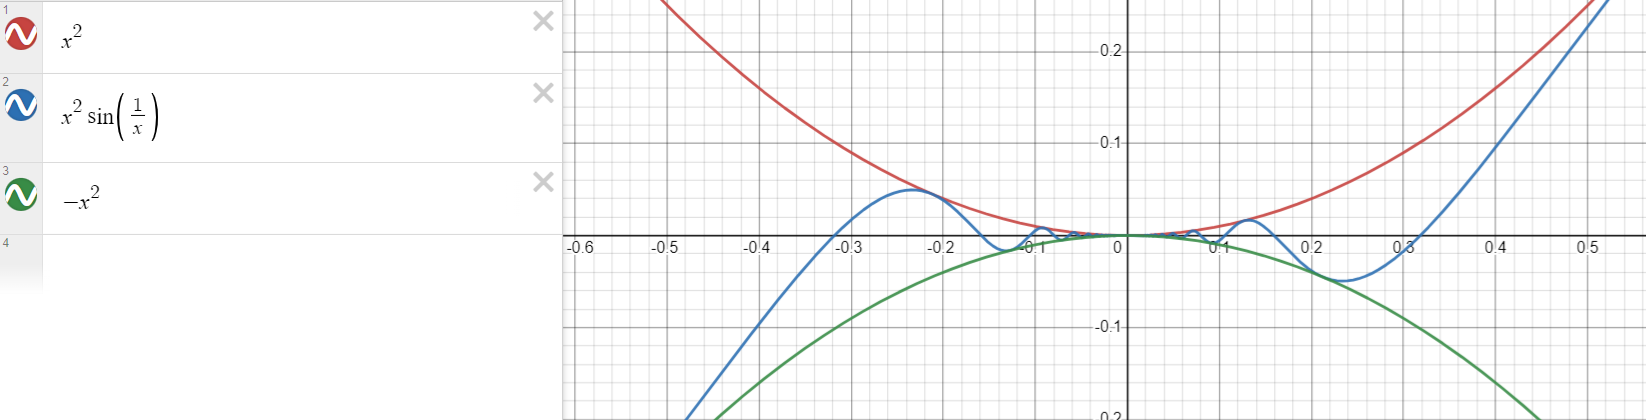
\includegraphics[width=0.99\linewidth]{tasks/task10/image.png}
\end{figure}
 
$f$ дифференцируема по Фреше в $x \neq 0$ (по правилу Лейбница):
\[\begin{aligned}
& {(x + h)}^{2} = x^2 +2xh+ \bar{o}(|h|)\\
& \sin{\frac{1}{x+h}} = \sin{\frac{1}{x}} + \frac{-1}{x^2} \cos{\frac{1}{x}}h + \bar{o}(|h|)
\end{aligned}\]
$|f(x)| \leq x^2 \implies f^{\prime}(0)=0$ и $f(x)-f(0)=f(x) =\bar{o}(|x|), |x| \rightarrow 0 $
то есть f диф. по Фреше в 0, тогда и на всем $\mathbb{R}$

Предположим противное: $f$ строго дифференцируемо в $0$.

По определению,  для любого $\varepsilon>0$ существует $\delta>0$ такое, что для любых $x_1, x_2 \in O_\delta\left(x_0\right)$ выполнено
\[\begin{aligned}
&|f\left(x_1\right)-f\left(x_2\right)-A\left(x_1-x_2\right)|\leq \varepsilon|x_1-x_2| \\
&f^{\prime}(0)=0 \implies |f\left(x_1\right)-f\left(x_2\right)|\leq \varepsilon|x_1-x_2|\leq 2\varepsilon \delta \\
& x\neq 0:  f^{\prime}(x)=2 x \sin \frac{1}{x}+x^2 \cos \frac{1}{x}\left(-1 \cdot \frac{1}{x^2}\right)=2 x \sin \left(\frac{1}{x}\right)-\cos \frac{1}{x} \nrightarrow 0, x \rightarrow 0 \\
& \text{потому что } \lim _{x \rightarrow 0} x \sin \frac{1}{x}=0 \text{ и } \lim _{x \rightarrow 0} \cos \frac{1}{x} \text{ не существует.} \\
& \text{Тогда }\exists \xi_n \rightarrow 0 \quad\left|f^{\prime}\left(\xi_n\right)\right| \geqslant c>0 \\
& f\left(\xi_n+h_n\right)-f\left(\xi_n\right)=f^{\prime}\left(\xi_n\right) h_n+\bar{o}\left(h_n\right) \text{ (по опр. диф. по Фреше)}\\
& h_n \longrightarrow 0 :\\
& \left|f\left(\xi_n+h_n\right)-f\left(\xi_n\right)\right| \geqslant C\left|h_n\right|
\end{aligned}\]
Получили противоречие. $f$ не является строго дифференцируемой в нуле.
\end{task}

\begin{task}
Привести пример функции $f: \mathbb{R} \rightarrow \mathbb{R}$, всюду дифференцируемой по Фреше, но не строго дифференцируемой в нуле.

\textbf{Доказательство:}
Рассмотрим функцию $f$:
\[
f(x)= \begin{cases}0, & x=0 \\ x^2 \sin \left(\frac{1}{x}\right), & x \neq 0\end{cases} 
\]

\begin{figure}[h!]
\centering
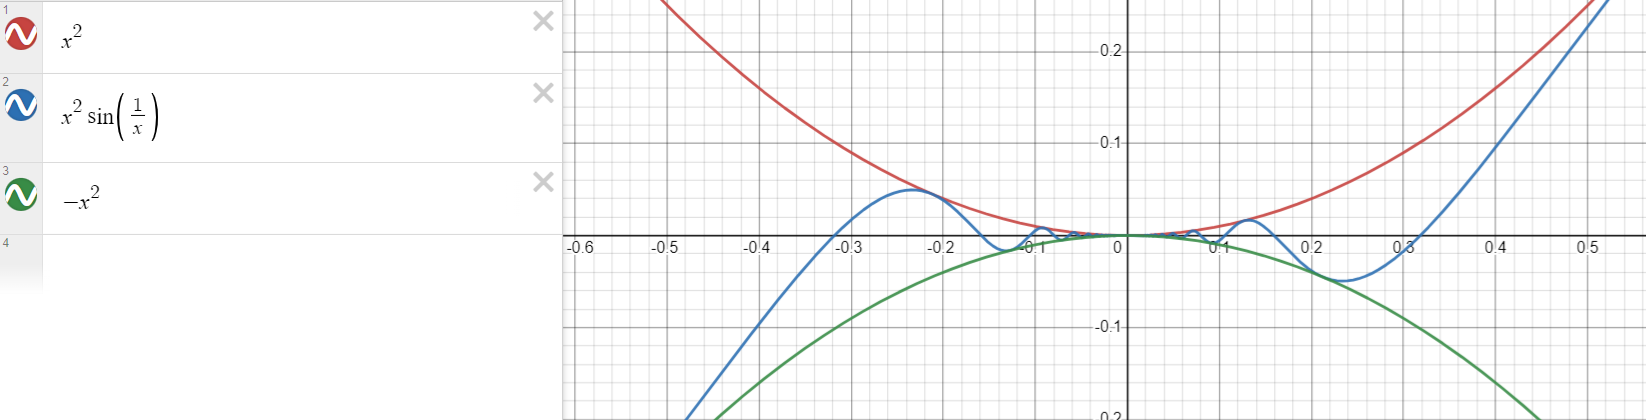
\includegraphics[width=0.99\linewidth]{tasks/task10/image.png}
\end{figure}
 
$f$ дифференцируема по Фреше в $x \neq 0$ (по правилу Лейбница):
\[\begin{aligned}
& {(x + h)}^{2} = x^2 +2xh+ \bar{o}(|h|)\\
& \sin{\frac{1}{x+h}} = \sin{\frac{1}{x}} + \frac{-1}{x^2} \cos{\frac{1}{x}}h + \bar{o}(|h|)
\end{aligned}\]
$|f(x)| \leq x^2 \implies f^{\prime}(0)=0$ и $f(x)-f(0)=f(x) =\bar{o}(|x|), |x| \rightarrow 0 $
то есть f диф. по Фреше в 0, тогда и на всем $\mathbb{R}$

Предположим противное: $f$ строго дифференцируемо в $0$.

По определению,  для любого $\varepsilon>0$ существует $\delta>0$ такое, что для любых $x_1, x_2 \in O_\delta\left(x_0\right)$ выполнено
\[\begin{aligned}
&|f\left(x_1\right)-f\left(x_2\right)-A\left(x_1-x_2\right)|\leq \varepsilon|x_1-x_2| \\
&f^{\prime}(0)=0 \implies |f\left(x_1\right)-f\left(x_2\right)|\leq \varepsilon|x_1-x_2|\leq 2\varepsilon \delta \\
& x\neq 0:  f^{\prime}(x)=2 x \sin \frac{1}{x}+x^2 \cos \frac{1}{x}\left(-1 \cdot \frac{1}{x^2}\right)=2 x \sin \left(\frac{1}{x}\right)-\cos \frac{1}{x} \nrightarrow 0, x \rightarrow 0 \\
& \text{потому что } \lim _{x \rightarrow 0} x \sin \frac{1}{x}=0 \text{ и } \lim _{x \rightarrow 0} \cos \frac{1}{x} \text{ не существует.} \\
& \text{Тогда }\exists \xi_n \rightarrow 0 \quad\left|f^{\prime}\left(\xi_n\right)\right| \geqslant c>0 \\
& f\left(\xi_n+h_n\right)-f\left(\xi_n\right)=f^{\prime}\left(\xi_n\right) h_n+\bar{o}\left(h_n\right) \text{ (по опр. диф. по Фреше)}\\
& h_n \longrightarrow 0 :\\
& \left|f\left(\xi_n+h_n\right)-f\left(\xi_n\right)\right| \geqslant C\left|h_n\right|
\end{aligned}\]
Получили противоречие. $f$ не является строго дифференцируемой в нуле.
\end{task}

\begin{task}
Привести пример функции $f: \mathbb{R} \rightarrow \mathbb{R}$, всюду дифференцируемой по Фреше, но не строго дифференцируемой в нуле.

\textbf{Доказательство:}
Рассмотрим функцию $f$:
\[
f(x)= \begin{cases}0, & x=0 \\ x^2 \sin \left(\frac{1}{x}\right), & x \neq 0\end{cases} 
\]

\begin{figure}[h!]
\centering
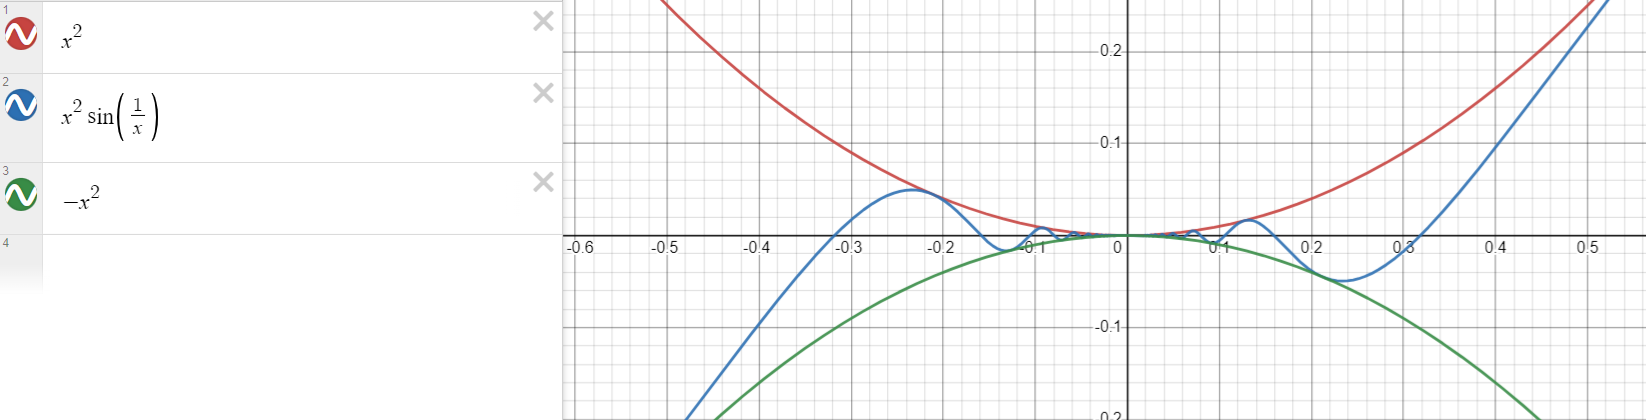
\includegraphics[width=0.99\linewidth]{tasks/task10/image.png}
\end{figure}
 
$f$ дифференцируема по Фреше в $x \neq 0$ (по правилу Лейбница):
\[\begin{aligned}
& {(x + h)}^{2} = x^2 +2xh+ \bar{o}(|h|)\\
& \sin{\frac{1}{x+h}} = \sin{\frac{1}{x}} + \frac{-1}{x^2} \cos{\frac{1}{x}}h + \bar{o}(|h|)
\end{aligned}\]
$|f(x)| \leq x^2 \implies f^{\prime}(0)=0$ и $f(x)-f(0)=f(x) =\bar{o}(|x|), |x| \rightarrow 0 $
то есть f диф. по Фреше в 0, тогда и на всем $\mathbb{R}$

Предположим противное: $f$ строго дифференцируемо в $0$.

По определению,  для любого $\varepsilon>0$ существует $\delta>0$ такое, что для любых $x_1, x_2 \in O_\delta\left(x_0\right)$ выполнено
\[\begin{aligned}
&|f\left(x_1\right)-f\left(x_2\right)-A\left(x_1-x_2\right)|\leq \varepsilon|x_1-x_2| \\
&f^{\prime}(0)=0 \implies |f\left(x_1\right)-f\left(x_2\right)|\leq \varepsilon|x_1-x_2|\leq 2\varepsilon \delta \\
& x\neq 0:  f^{\prime}(x)=2 x \sin \frac{1}{x}+x^2 \cos \frac{1}{x}\left(-1 \cdot \frac{1}{x^2}\right)=2 x \sin \left(\frac{1}{x}\right)-\cos \frac{1}{x} \nrightarrow 0, x \rightarrow 0 \\
& \text{потому что } \lim _{x \rightarrow 0} x \sin \frac{1}{x}=0 \text{ и } \lim _{x \rightarrow 0} \cos \frac{1}{x} \text{ не существует.} \\
& \text{Тогда }\exists \xi_n \rightarrow 0 \quad\left|f^{\prime}\left(\xi_n\right)\right| \geqslant c>0 \\
& f\left(\xi_n+h_n\right)-f\left(\xi_n\right)=f^{\prime}\left(\xi_n\right) h_n+\bar{o}\left(h_n\right) \text{ (по опр. диф. по Фреше)}\\
& h_n \longrightarrow 0 :\\
& \left|f\left(\xi_n+h_n\right)-f\left(\xi_n\right)\right| \geqslant C\left|h_n\right|
\end{aligned}\]
Получили противоречие. $f$ не является строго дифференцируемой в нуле.
\end{task}

\begin{task}
Пусть $A: l_2 \rightarrow l_2$,
$$
A\left(x_1, x_2, \ldots, x_n, \ldots\right)=\left(x_1, x_2 / 2, \ldots, x_n / n, \ldots\right),
$$
$\left(y_1, \ldots, y_n, \ldots\right) \in l_2 \backslash \operatorname{Im} A$ (почему такая точка существует?). Рассмотрим задачу
$$
\sum_{n=1}^{\infty} y_n x_n \rightarrow \inf , \quad A\left(x_1, x_2, \ldots, x_n, \ldots\right)=0 .
$$

Какая точка будет точкой минимума в этой задаче? Показать, что для этой задачи принцип Лагранжа неверен. Какое из условий теоремы о необходимом условии локального минимума здесь не выполнено?
\vspace{1cm}

\textbf{Решение.} 

1) В качестве точки $y$ можно взять последовательность 
$(1,1 / 2, \ldots, 1 / n, \ldots) \in l_2$. Если $A x=y$, то $x_n=1$ для любого $n \in \mathbb{N}$, но $(1, \ldots, 1, \ldots) \notin l_2$.
\vspace{0.5cm}

2) Если $A\left(x_1, x_2, \ldots, x_n, \ldots\right)=0$, то $\frac{x_n}{n}=0$ для любого $n$. Значит, $x=0$-единственная допустимая точка, она же и будет точкой минимума.
\vspace{0.5cm}

3) Пусть $f_0(x)=\sum_{n=1}^{\infty} y_n x_n, F(x)=A(x)$. Тогда $f_0^{\prime}(x)[h]=\sum_{n=1}^{\infty} y_n h_n, F^{\prime}(x)[h]=A(h)=$ $\left(h_1, h_2 / 2, \ldots, h_n / n, \ldots\right)$. Если $z^*$ - линейный непрерывный функционал на $l_2$, то существует вектор $z=\left(z_1, \ldots, z_n, \ldots\right) \in l_2$ такой, что $z^*(x)=\sum_{n=1}^{\infty} z_n x_n$.

Таким образом, если принцип Лагранжа выполнен, то существуют $\lambda_0 \in \mathbb{R}$ и $z \in l_2$, одновременно не равные нулю, такие, что для любого $h \in l_2$ выполнено
$$
\lambda_0 \sum_{n=1}^{\infty} y_n h_n+\sum_{n=1}^{\infty} z_n \frac{h_n}{n}=0 .
$$

Значит, $\lambda_0 y_n+\frac{z_n}{n}=0, n \in \mathbb{N}$. Если $\lambda_0 \neq 0$, то $y_n=-\frac{z_n}{\lambda_0 n}$, то есть $y=A\left(-z / \lambda_0\right)$. Но $y \notin \operatorname{Im} A$ - противоречие. Если $\lambda_0=0$, то $\frac{z_n}{n}=0$ для любого $n$, поэтому $z=0$. Получили, что оба множителя Лагранжа нулевые.
\vspace{0.5cm}

4) Пространства $X=Y=l_2$ банаховы, $f_0$ и $F$ непрерывно дифференцируемы (это линейные непрерывные отображения). Но $\operatorname{Im} F^{\prime}(0)=\operatorname{Im} A$ незамкнут (он всюду плотен в $l_2$, но не совпадает с $l_2$ ).

\end{task}

\begin{task}
Привести пример функции $f: \mathbb{R} \rightarrow \mathbb{R}$, всюду дифференцируемой по Фреше, но не строго дифференцируемой в нуле.

\textbf{Доказательство:}
Рассмотрим функцию $f$:
\[
f(x)= \begin{cases}0, & x=0 \\ x^2 \sin \left(\frac{1}{x}\right), & x \neq 0\end{cases} 
\]

\begin{figure}[h!]
\centering
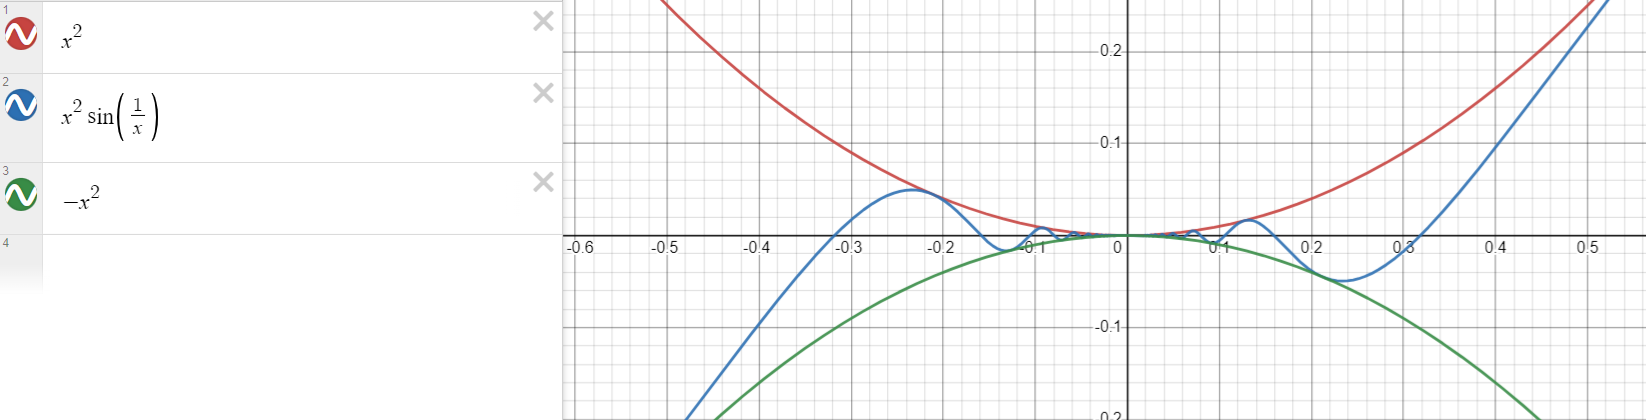
\includegraphics[width=0.99\linewidth]{tasks/task10/image.png}
\end{figure}
 
$f$ дифференцируема по Фреше в $x \neq 0$ (по правилу Лейбница):
\[\begin{aligned}
& {(x + h)}^{2} = x^2 +2xh+ \bar{o}(|h|)\\
& \sin{\frac{1}{x+h}} = \sin{\frac{1}{x}} + \frac{-1}{x^2} \cos{\frac{1}{x}}h + \bar{o}(|h|)
\end{aligned}\]
$|f(x)| \leq x^2 \implies f^{\prime}(0)=0$ и $f(x)-f(0)=f(x) =\bar{o}(|x|), |x| \rightarrow 0 $
то есть f диф. по Фреше в 0, тогда и на всем $\mathbb{R}$

Предположим противное: $f$ строго дифференцируемо в $0$.

По определению,  для любого $\varepsilon>0$ существует $\delta>0$ такое, что для любых $x_1, x_2 \in O_\delta\left(x_0\right)$ выполнено
\[\begin{aligned}
&|f\left(x_1\right)-f\left(x_2\right)-A\left(x_1-x_2\right)|\leq \varepsilon|x_1-x_2| \\
&f^{\prime}(0)=0 \implies |f\left(x_1\right)-f\left(x_2\right)|\leq \varepsilon|x_1-x_2|\leq 2\varepsilon \delta \\
& x\neq 0:  f^{\prime}(x)=2 x \sin \frac{1}{x}+x^2 \cos \frac{1}{x}\left(-1 \cdot \frac{1}{x^2}\right)=2 x \sin \left(\frac{1}{x}\right)-\cos \frac{1}{x} \nrightarrow 0, x \rightarrow 0 \\
& \text{потому что } \lim _{x \rightarrow 0} x \sin \frac{1}{x}=0 \text{ и } \lim _{x \rightarrow 0} \cos \frac{1}{x} \text{ не существует.} \\
& \text{Тогда }\exists \xi_n \rightarrow 0 \quad\left|f^{\prime}\left(\xi_n\right)\right| \geqslant c>0 \\
& f\left(\xi_n+h_n\right)-f\left(\xi_n\right)=f^{\prime}\left(\xi_n\right) h_n+\bar{o}\left(h_n\right) \text{ (по опр. диф. по Фреше)}\\
& h_n \longrightarrow 0 :\\
& \left|f\left(\xi_n+h_n\right)-f\left(\xi_n\right)\right| \geqslant C\left|h_n\right|
\end{aligned}\]
Получили противоречие. $f$ не является строго дифференцируемой в нуле.
\end{task}

\begin{task}

    Пусть $\hat{x} \in M$ - точка локального минимума в задаче
    
    $$
    \left\{\begin{array}{l}
    f_{0}(x) \rightarrow \inf \\
    x \in M
    \end{array}\right.
    $$\\
    функция $f_{0}$ дифференцируема по Гато в точке $\hat{x}$. \\
    Верно ли, что тогда $f_{0}^{\prime}(\hat{x})[h]=0$ для любого $h \in T_{\hat{x}} M$ ?\\
    \textbf{Ответ:} нет, неверно.\\
    \textbf{Пример:}
    Пусть $M=\left\{(x, y): y=x^{2}\right\}$ (т.е. парабола на плоскости),
    $$
    f_{0}(x, y)= \begin{cases}0, & \text { если } y=x^{2} \\ x, & \text { иначе. }\end{cases}
    $$
    
    Тогда $f_0 = 0$ на M, поэтому $(0,0)$ - точка минимума $f_{0}$ на $M$. При $f_{0}(t h, t g)=t h$ при малых $t$ (если t < $\frac{g}{h}$, то $t^2h^2 < tg)$, поэтому $f_{0}^{\prime}(0,0)[(h, g)]=h$.\\ 
    Касательный вектор в $(0,0)$ к параболе $M$ имеет вид $(h, 0)$, так что на нем производная равна $h \neq 0$. 
    \end{task}
\begin{task}
Привести пример функции $f: \mathbb{R} \rightarrow \mathbb{R}$, всюду дифференцируемой по Фреше, но не строго дифференцируемой в нуле.

\textbf{Доказательство:}
Рассмотрим функцию $f$:
\[
f(x)= \begin{cases}0, & x=0 \\ x^2 \sin \left(\frac{1}{x}\right), & x \neq 0\end{cases} 
\]

\begin{figure}[h!]
\centering
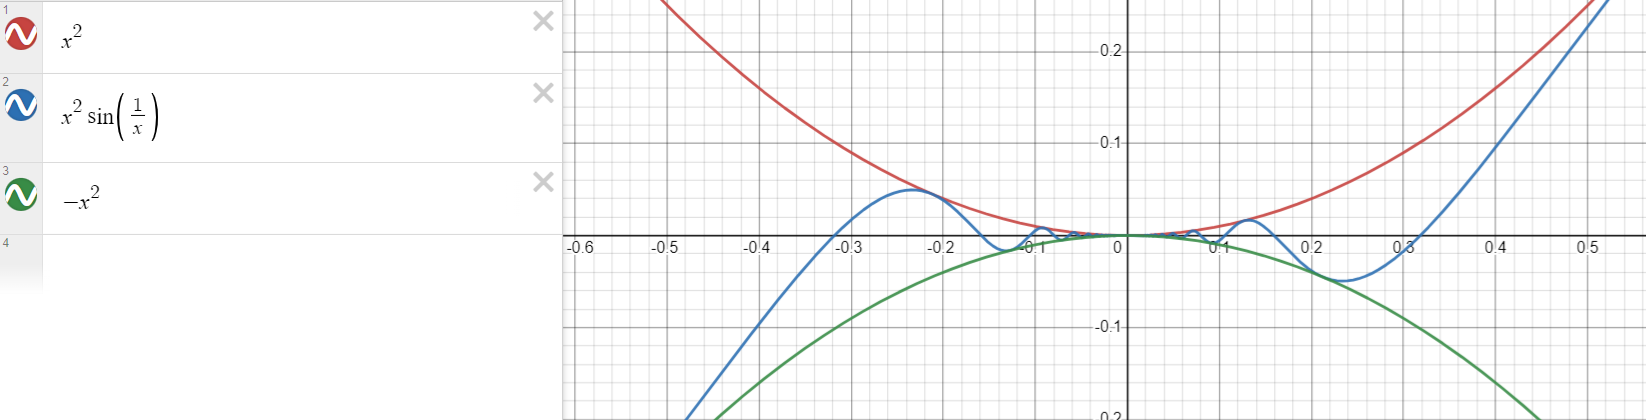
\includegraphics[width=0.99\linewidth]{tasks/task10/image.png}
\end{figure}
 
$f$ дифференцируема по Фреше в $x \neq 0$ (по правилу Лейбница):
\[\begin{aligned}
& {(x + h)}^{2} = x^2 +2xh+ \bar{o}(|h|)\\
& \sin{\frac{1}{x+h}} = \sin{\frac{1}{x}} + \frac{-1}{x^2} \cos{\frac{1}{x}}h + \bar{o}(|h|)
\end{aligned}\]
$|f(x)| \leq x^2 \implies f^{\prime}(0)=0$ и $f(x)-f(0)=f(x) =\bar{o}(|x|), |x| \rightarrow 0 $
то есть f диф. по Фреше в 0, тогда и на всем $\mathbb{R}$

Предположим противное: $f$ строго дифференцируемо в $0$.

По определению,  для любого $\varepsilon>0$ существует $\delta>0$ такое, что для любых $x_1, x_2 \in O_\delta\left(x_0\right)$ выполнено
\[\begin{aligned}
&|f\left(x_1\right)-f\left(x_2\right)-A\left(x_1-x_2\right)|\leq \varepsilon|x_1-x_2| \\
&f^{\prime}(0)=0 \implies |f\left(x_1\right)-f\left(x_2\right)|\leq \varepsilon|x_1-x_2|\leq 2\varepsilon \delta \\
& x\neq 0:  f^{\prime}(x)=2 x \sin \frac{1}{x}+x^2 \cos \frac{1}{x}\left(-1 \cdot \frac{1}{x^2}\right)=2 x \sin \left(\frac{1}{x}\right)-\cos \frac{1}{x} \nrightarrow 0, x \rightarrow 0 \\
& \text{потому что } \lim _{x \rightarrow 0} x \sin \frac{1}{x}=0 \text{ и } \lim _{x \rightarrow 0} \cos \frac{1}{x} \text{ не существует.} \\
& \text{Тогда }\exists \xi_n \rightarrow 0 \quad\left|f^{\prime}\left(\xi_n\right)\right| \geqslant c>0 \\
& f\left(\xi_n+h_n\right)-f\left(\xi_n\right)=f^{\prime}\left(\xi_n\right) h_n+\bar{o}\left(h_n\right) \text{ (по опр. диф. по Фреше)}\\
& h_n \longrightarrow 0 :\\
& \left|f\left(\xi_n+h_n\right)-f\left(\xi_n\right)\right| \geqslant C\left|h_n\right|
\end{aligned}\]
Получили противоречие. $f$ не является строго дифференцируемой в нуле.
\end{task}

\begin{task}
Задача 18. Привести пример такой задачи выпуклого программирования, что допустимая $\hat{x}-$ не есть точка минимума, но существует ненулевой набор $\left(\lambda_{0}, \ldots, \lambda_{m}\right)$, удовлетворяющий условиям а)-с) теоремы Куна-Таккера.

Если $\hat{x}$ - решение задачи на минимум $f_{0}(x)$ при условии $f_{1}(\hat{x})=0, f_{2}(\hat{x})=0$, где функционалы выпуклы, то для функции Лагранжа $\mathcal{L}(x)=$ $\sum_{j \geq 0} \lambda_{j} f_{j}(x)$ справедливы условия

a) минимум функции Лагранжа достигается на решении;

b) $\lambda_{j} f_{j}(\hat{x})=0, j \geq 1$;

c) $\lambda_{j} \geq 0, j \geq 0$.

Пусть $x=\left(x_{1}, x_{2}\right) \in \mathbb{R}^{2}, f_{1}(x)=x_{1}, f_{2}(x)=x_{2}$, а $f_{0}(x)=x_{1}^{2}+\left(x_{2}-1\right)^{2}$. Тогда для функции Лагранжа $\mathcal{L}(x)=f_{1}(x)+f_{2}(x)$ имеем: точка $\hat{x}=(0,0)$ - допустимая, условия а)-с) выполнены, но минимум $f_{0}(x)$ достигается в точке $(0,1)$.


\end{task}

\begin{task}
Привести пример функции $f: \mathbb{R} \rightarrow \mathbb{R}$, всюду дифференцируемой по Фреше, но не строго дифференцируемой в нуле.

\textbf{Доказательство:}
Рассмотрим функцию $f$:
\[
f(x)= \begin{cases}0, & x=0 \\ x^2 \sin \left(\frac{1}{x}\right), & x \neq 0\end{cases} 
\]

\begin{figure}[h!]
\centering
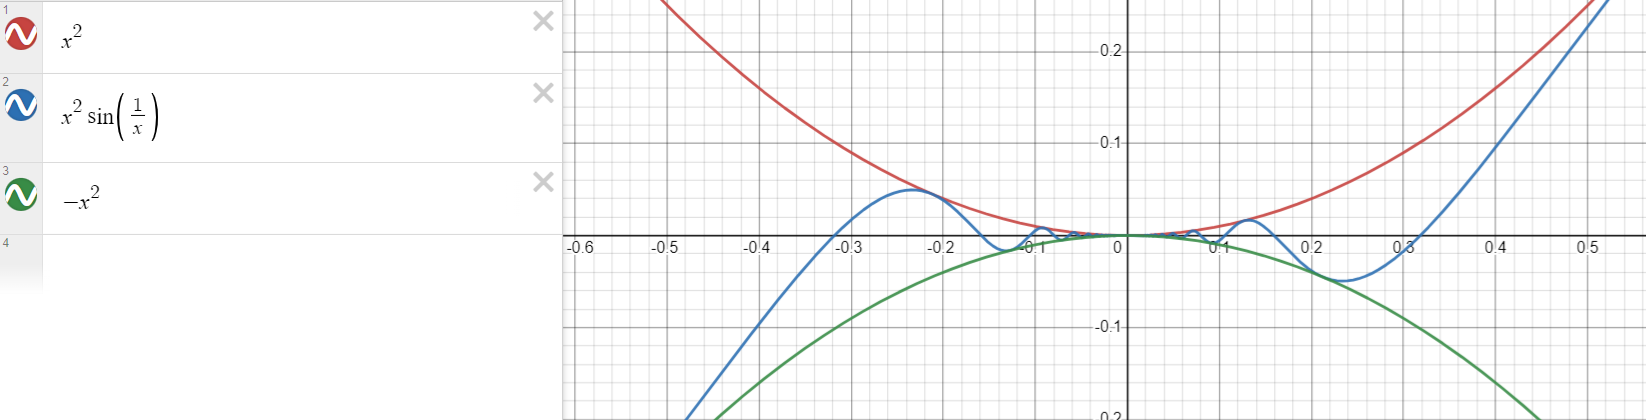
\includegraphics[width=0.99\linewidth]{tasks/task10/image.png}
\end{figure}
 
$f$ дифференцируема по Фреше в $x \neq 0$ (по правилу Лейбница):
\[\begin{aligned}
& {(x + h)}^{2} = x^2 +2xh+ \bar{o}(|h|)\\
& \sin{\frac{1}{x+h}} = \sin{\frac{1}{x}} + \frac{-1}{x^2} \cos{\frac{1}{x}}h + \bar{o}(|h|)
\end{aligned}\]
$|f(x)| \leq x^2 \implies f^{\prime}(0)=0$ и $f(x)-f(0)=f(x) =\bar{o}(|x|), |x| \rightarrow 0 $
то есть f диф. по Фреше в 0, тогда и на всем $\mathbb{R}$

Предположим противное: $f$ строго дифференцируемо в $0$.

По определению,  для любого $\varepsilon>0$ существует $\delta>0$ такое, что для любых $x_1, x_2 \in O_\delta\left(x_0\right)$ выполнено
\[\begin{aligned}
&|f\left(x_1\right)-f\left(x_2\right)-A\left(x_1-x_2\right)|\leq \varepsilon|x_1-x_2| \\
&f^{\prime}(0)=0 \implies |f\left(x_1\right)-f\left(x_2\right)|\leq \varepsilon|x_1-x_2|\leq 2\varepsilon \delta \\
& x\neq 0:  f^{\prime}(x)=2 x \sin \frac{1}{x}+x^2 \cos \frac{1}{x}\left(-1 \cdot \frac{1}{x^2}\right)=2 x \sin \left(\frac{1}{x}\right)-\cos \frac{1}{x} \nrightarrow 0, x \rightarrow 0 \\
& \text{потому что } \lim _{x \rightarrow 0} x \sin \frac{1}{x}=0 \text{ и } \lim _{x \rightarrow 0} \cos \frac{1}{x} \text{ не существует.} \\
& \text{Тогда }\exists \xi_n \rightarrow 0 \quad\left|f^{\prime}\left(\xi_n\right)\right| \geqslant c>0 \\
& f\left(\xi_n+h_n\right)-f\left(\xi_n\right)=f^{\prime}\left(\xi_n\right) h_n+\bar{o}\left(h_n\right) \text{ (по опр. диф. по Фреше)}\\
& h_n \longrightarrow 0 :\\
& \left|f\left(\xi_n+h_n\right)-f\left(\xi_n\right)\right| \geqslant C\left|h_n\right|
\end{aligned}\]
Получили противоречие. $f$ не является строго дифференцируемой в нуле.
\end{task}

\begin{task}
Привести пример функции $f: \mathbb{R} \rightarrow \mathbb{R}$, всюду дифференцируемой по Фреше, но не строго дифференцируемой в нуле.

\textbf{Доказательство:}
Рассмотрим функцию $f$:
\[
f(x)= \begin{cases}0, & x=0 \\ x^2 \sin \left(\frac{1}{x}\right), & x \neq 0\end{cases} 
\]

\begin{figure}[h!]
\centering
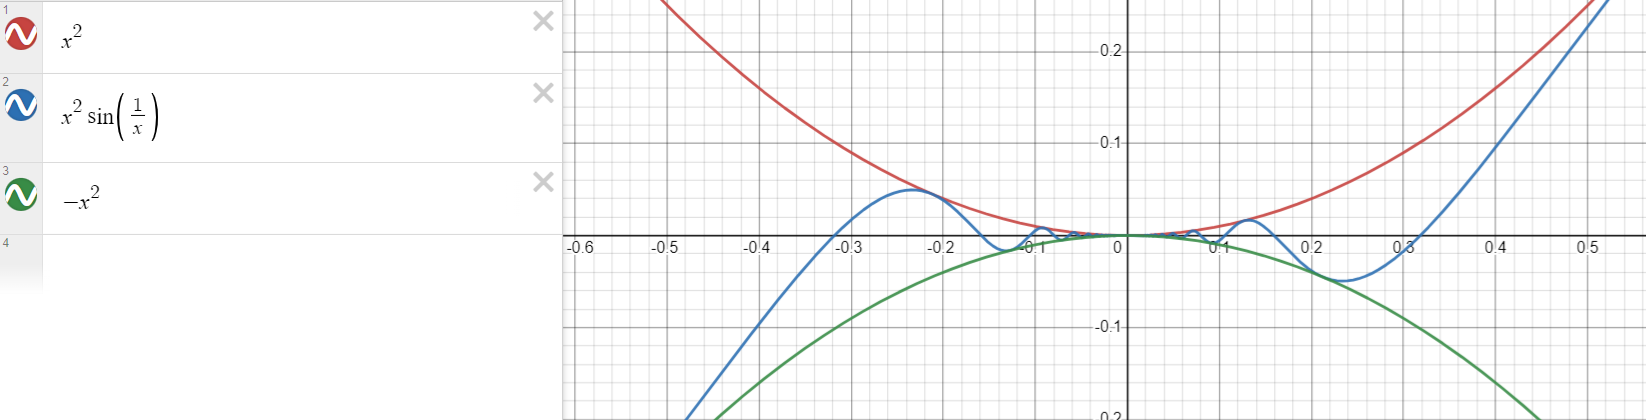
\includegraphics[width=0.99\linewidth]{tasks/task10/image.png}
\end{figure}
 
$f$ дифференцируема по Фреше в $x \neq 0$ (по правилу Лейбница):
\[\begin{aligned}
& {(x + h)}^{2} = x^2 +2xh+ \bar{o}(|h|)\\
& \sin{\frac{1}{x+h}} = \sin{\frac{1}{x}} + \frac{-1}{x^2} \cos{\frac{1}{x}}h + \bar{o}(|h|)
\end{aligned}\]
$|f(x)| \leq x^2 \implies f^{\prime}(0)=0$ и $f(x)-f(0)=f(x) =\bar{o}(|x|), |x| \rightarrow 0 $
то есть f диф. по Фреше в 0, тогда и на всем $\mathbb{R}$

Предположим противное: $f$ строго дифференцируемо в $0$.

По определению,  для любого $\varepsilon>0$ существует $\delta>0$ такое, что для любых $x_1, x_2 \in O_\delta\left(x_0\right)$ выполнено
\[\begin{aligned}
&|f\left(x_1\right)-f\left(x_2\right)-A\left(x_1-x_2\right)|\leq \varepsilon|x_1-x_2| \\
&f^{\prime}(0)=0 \implies |f\left(x_1\right)-f\left(x_2\right)|\leq \varepsilon|x_1-x_2|\leq 2\varepsilon \delta \\
& x\neq 0:  f^{\prime}(x)=2 x \sin \frac{1}{x}+x^2 \cos \frac{1}{x}\left(-1 \cdot \frac{1}{x^2}\right)=2 x \sin \left(\frac{1}{x}\right)-\cos \frac{1}{x} \nrightarrow 0, x \rightarrow 0 \\
& \text{потому что } \lim _{x \rightarrow 0} x \sin \frac{1}{x}=0 \text{ и } \lim _{x \rightarrow 0} \cos \frac{1}{x} \text{ не существует.} \\
& \text{Тогда }\exists \xi_n \rightarrow 0 \quad\left|f^{\prime}\left(\xi_n\right)\right| \geqslant c>0 \\
& f\left(\xi_n+h_n\right)-f\left(\xi_n\right)=f^{\prime}\left(\xi_n\right) h_n+\bar{o}\left(h_n\right) \text{ (по опр. диф. по Фреше)}\\
& h_n \longrightarrow 0 :\\
& \left|f\left(\xi_n+h_n\right)-f\left(\xi_n\right)\right| \geqslant C\left|h_n\right|
\end{aligned}\]
Получили противоречие. $f$ не является строго дифференцируемой в нуле.
\end{task}

\begin{task}
Привести пример функции $f: \mathbb{R} \rightarrow \mathbb{R}$, всюду дифференцируемой по Фреше, но не строго дифференцируемой в нуле.

\textbf{Доказательство:}
Рассмотрим функцию $f$:
\[
f(x)= \begin{cases}0, & x=0 \\ x^2 \sin \left(\frac{1}{x}\right), & x \neq 0\end{cases} 
\]

\begin{figure}[h!]
\centering
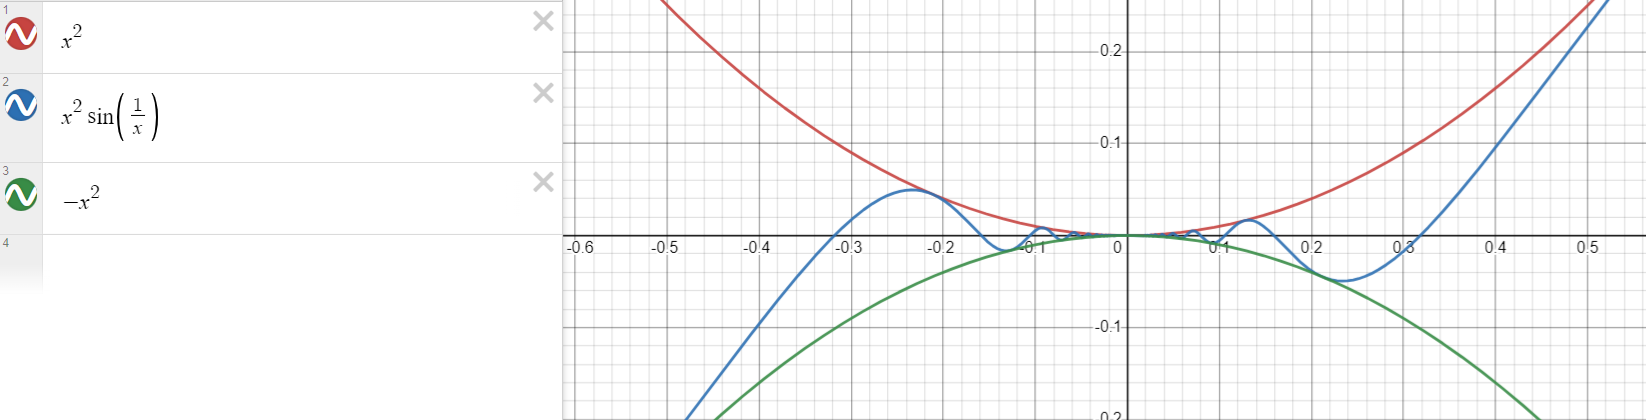
\includegraphics[width=0.99\linewidth]{tasks/task10/image.png}
\end{figure}
 
$f$ дифференцируема по Фреше в $x \neq 0$ (по правилу Лейбница):
\[\begin{aligned}
& {(x + h)}^{2} = x^2 +2xh+ \bar{o}(|h|)\\
& \sin{\frac{1}{x+h}} = \sin{\frac{1}{x}} + \frac{-1}{x^2} \cos{\frac{1}{x}}h + \bar{o}(|h|)
\end{aligned}\]
$|f(x)| \leq x^2 \implies f^{\prime}(0)=0$ и $f(x)-f(0)=f(x) =\bar{o}(|x|), |x| \rightarrow 0 $
то есть f диф. по Фреше в 0, тогда и на всем $\mathbb{R}$

Предположим противное: $f$ строго дифференцируемо в $0$.

По определению,  для любого $\varepsilon>0$ существует $\delta>0$ такое, что для любых $x_1, x_2 \in O_\delta\left(x_0\right)$ выполнено
\[\begin{aligned}
&|f\left(x_1\right)-f\left(x_2\right)-A\left(x_1-x_2\right)|\leq \varepsilon|x_1-x_2| \\
&f^{\prime}(0)=0 \implies |f\left(x_1\right)-f\left(x_2\right)|\leq \varepsilon|x_1-x_2|\leq 2\varepsilon \delta \\
& x\neq 0:  f^{\prime}(x)=2 x \sin \frac{1}{x}+x^2 \cos \frac{1}{x}\left(-1 \cdot \frac{1}{x^2}\right)=2 x \sin \left(\frac{1}{x}\right)-\cos \frac{1}{x} \nrightarrow 0, x \rightarrow 0 \\
& \text{потому что } \lim _{x \rightarrow 0} x \sin \frac{1}{x}=0 \text{ и } \lim _{x \rightarrow 0} \cos \frac{1}{x} \text{ не существует.} \\
& \text{Тогда }\exists \xi_n \rightarrow 0 \quad\left|f^{\prime}\left(\xi_n\right)\right| \geqslant c>0 \\
& f\left(\xi_n+h_n\right)-f\left(\xi_n\right)=f^{\prime}\left(\xi_n\right) h_n+\bar{o}\left(h_n\right) \text{ (по опр. диф. по Фреше)}\\
& h_n \longrightarrow 0 :\\
& \left|f\left(\xi_n+h_n\right)-f\left(\xi_n\right)\right| \geqslant C\left|h_n\right|
\end{aligned}\]
Получили противоречие. $f$ не является строго дифференцируемой в нуле.
\end{task}

\begin{task}
Привести пример функции $f: \mathbb{R} \rightarrow \mathbb{R}$, всюду дифференцируемой по Фреше, но не строго дифференцируемой в нуле.

\textbf{Доказательство:}
Рассмотрим функцию $f$:
\[
f(x)= \begin{cases}0, & x=0 \\ x^2 \sin \left(\frac{1}{x}\right), & x \neq 0\end{cases} 
\]

\begin{figure}[h!]
\centering
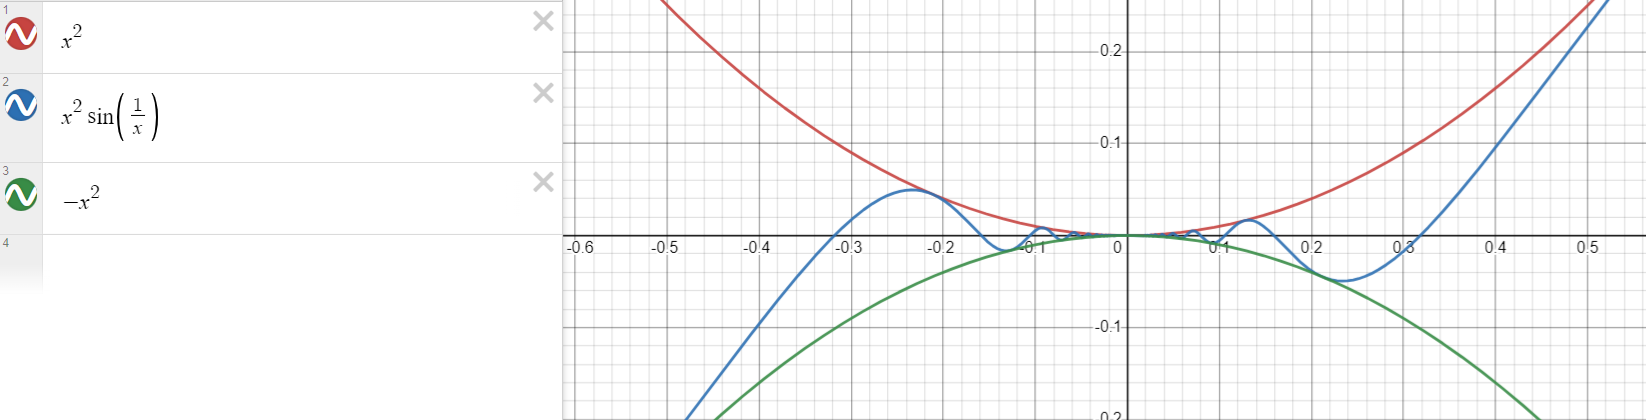
\includegraphics[width=0.99\linewidth]{tasks/task10/image.png}
\end{figure}
 
$f$ дифференцируема по Фреше в $x \neq 0$ (по правилу Лейбница):
\[\begin{aligned}
& {(x + h)}^{2} = x^2 +2xh+ \bar{o}(|h|)\\
& \sin{\frac{1}{x+h}} = \sin{\frac{1}{x}} + \frac{-1}{x^2} \cos{\frac{1}{x}}h + \bar{o}(|h|)
\end{aligned}\]
$|f(x)| \leq x^2 \implies f^{\prime}(0)=0$ и $f(x)-f(0)=f(x) =\bar{o}(|x|), |x| \rightarrow 0 $
то есть f диф. по Фреше в 0, тогда и на всем $\mathbb{R}$

Предположим противное: $f$ строго дифференцируемо в $0$.

По определению,  для любого $\varepsilon>0$ существует $\delta>0$ такое, что для любых $x_1, x_2 \in O_\delta\left(x_0\right)$ выполнено
\[\begin{aligned}
&|f\left(x_1\right)-f\left(x_2\right)-A\left(x_1-x_2\right)|\leq \varepsilon|x_1-x_2| \\
&f^{\prime}(0)=0 \implies |f\left(x_1\right)-f\left(x_2\right)|\leq \varepsilon|x_1-x_2|\leq 2\varepsilon \delta \\
& x\neq 0:  f^{\prime}(x)=2 x \sin \frac{1}{x}+x^2 \cos \frac{1}{x}\left(-1 \cdot \frac{1}{x^2}\right)=2 x \sin \left(\frac{1}{x}\right)-\cos \frac{1}{x} \nrightarrow 0, x \rightarrow 0 \\
& \text{потому что } \lim _{x \rightarrow 0} x \sin \frac{1}{x}=0 \text{ и } \lim _{x \rightarrow 0} \cos \frac{1}{x} \text{ не существует.} \\
& \text{Тогда }\exists \xi_n \rightarrow 0 \quad\left|f^{\prime}\left(\xi_n\right)\right| \geqslant c>0 \\
& f\left(\xi_n+h_n\right)-f\left(\xi_n\right)=f^{\prime}\left(\xi_n\right) h_n+\bar{o}\left(h_n\right) \text{ (по опр. диф. по Фреше)}\\
& h_n \longrightarrow 0 :\\
& \left|f\left(\xi_n+h_n\right)-f\left(\xi_n\right)\right| \geqslant C\left|h_n\right|
\end{aligned}\]
Получили противоречие. $f$ не является строго дифференцируемой в нуле.
\end{task}

\begin{task}
    Рассмотрим задачу $\int_0^\pi\left(\dot{x}^2-x^2-x^4\right) d t \rightarrow$ inf, $x(0)=x(\pi)=$ 0. Показать, что для $\hat{x}=0$ выполнено yсиленное условие Лежантра, условие Якоби, при этом $\hat{x}=0$ не является точкой слабого минимума.
    
    \textbf{Peшение.} Имеем $\hat{L}_{\dot{x} \dot{x}}(t)=2, \hat{L}_{\dot{x} x}=0, \hat{L}_{x x}=-2$. 3начит, выполнено усиленное условие Лежандра. Уравнение Якоби имеет вид $\ddot{h}+h=0$; его нетривиальное решение, зануляющееся при $t=0$, имеет вид $h(t)=a \sin t$, $a \neq 0$. Torда $h(t) \neq 0$ при $t \in(0, \pi)$, но $h(\pi)=0$. Значит, выполнено условие Якоби, но не усиленное.
    Boзьмем $x(t)=\varepsilon \sin t$. Toгдa
    $$
    \begin{gathered}
    \int_0^\pi\left(\dot{x}^2-x^2-x^4\right) d t=\varepsilon^2 \int_0^\pi\left(\cos ^2 t-\sin ^2 t\right) d t-\varepsilon^4 \int_0^\pi \sin ^4 t d t= \\
    =\varepsilon^2 \int_0^\pi \cos 2 t d t-\varepsilon^4 \int_0^\pi \sin ^4 t d t=-\varepsilon^4 \int_0^\pi \sin ^4 t d t<0 .
    \end{gathered}
    $$
    
    Так как $\varepsilon>0$ может быть сколь угодно мало, то слабого минимума нет.
\end{task}
\begin{task}
Привести пример функции $f: \mathbb{R} \rightarrow \mathbb{R}$, всюду дифференцируемой по Фреше, но не строго дифференцируемой в нуле.

\textbf{Доказательство:}
Рассмотрим функцию $f$:
\[
f(x)= \begin{cases}0, & x=0 \\ x^2 \sin \left(\frac{1}{x}\right), & x \neq 0\end{cases} 
\]

\begin{figure}[h!]
\centering
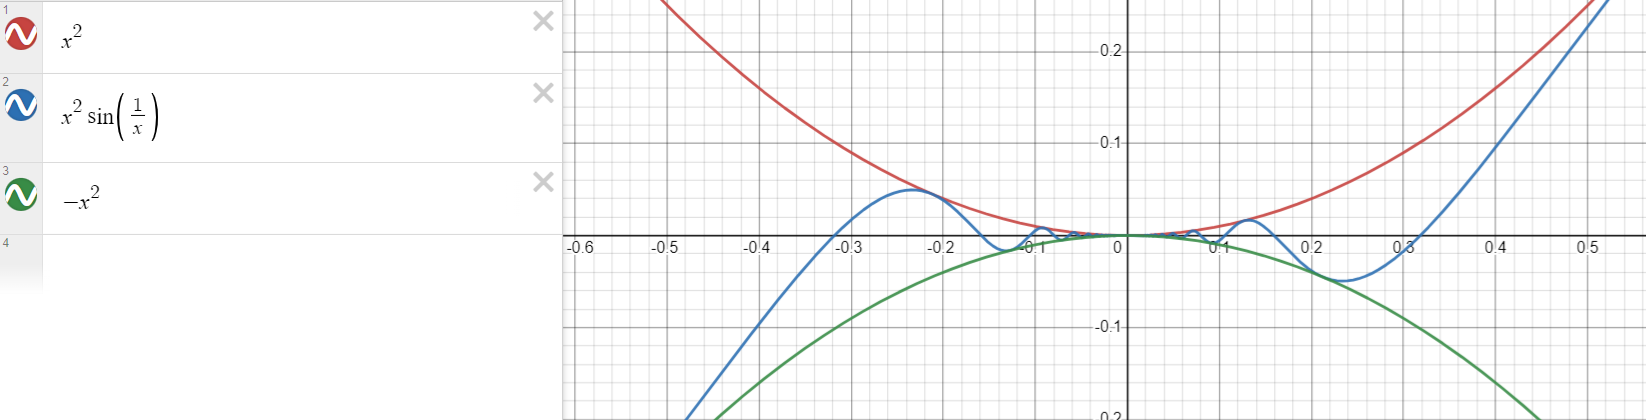
\includegraphics[width=0.99\linewidth]{tasks/task10/image.png}
\end{figure}
 
$f$ дифференцируема по Фреше в $x \neq 0$ (по правилу Лейбница):
\[\begin{aligned}
& {(x + h)}^{2} = x^2 +2xh+ \bar{o}(|h|)\\
& \sin{\frac{1}{x+h}} = \sin{\frac{1}{x}} + \frac{-1}{x^2} \cos{\frac{1}{x}}h + \bar{o}(|h|)
\end{aligned}\]
$|f(x)| \leq x^2 \implies f^{\prime}(0)=0$ и $f(x)-f(0)=f(x) =\bar{o}(|x|), |x| \rightarrow 0 $
то есть f диф. по Фреше в 0, тогда и на всем $\mathbb{R}$

Предположим противное: $f$ строго дифференцируемо в $0$.

По определению,  для любого $\varepsilon>0$ существует $\delta>0$ такое, что для любых $x_1, x_2 \in O_\delta\left(x_0\right)$ выполнено
\[\begin{aligned}
&|f\left(x_1\right)-f\left(x_2\right)-A\left(x_1-x_2\right)|\leq \varepsilon|x_1-x_2| \\
&f^{\prime}(0)=0 \implies |f\left(x_1\right)-f\left(x_2\right)|\leq \varepsilon|x_1-x_2|\leq 2\varepsilon \delta \\
& x\neq 0:  f^{\prime}(x)=2 x \sin \frac{1}{x}+x^2 \cos \frac{1}{x}\left(-1 \cdot \frac{1}{x^2}\right)=2 x \sin \left(\frac{1}{x}\right)-\cos \frac{1}{x} \nrightarrow 0, x \rightarrow 0 \\
& \text{потому что } \lim _{x \rightarrow 0} x \sin \frac{1}{x}=0 \text{ и } \lim _{x \rightarrow 0} \cos \frac{1}{x} \text{ не существует.} \\
& \text{Тогда }\exists \xi_n \rightarrow 0 \quad\left|f^{\prime}\left(\xi_n\right)\right| \geqslant c>0 \\
& f\left(\xi_n+h_n\right)-f\left(\xi_n\right)=f^{\prime}\left(\xi_n\right) h_n+\bar{o}\left(h_n\right) \text{ (по опр. диф. по Фреше)}\\
& h_n \longrightarrow 0 :\\
& \left|f\left(\xi_n+h_n\right)-f\left(\xi_n\right)\right| \geqslant C\left|h_n\right|
\end{aligned}\]
Получили противоречие. $f$ не является строго дифференцируемой в нуле.
\end{task}

\begin{task}
Привести пример функции $f: \mathbb{R} \rightarrow \mathbb{R}$, всюду дифференцируемой по Фреше, но не строго дифференцируемой в нуле.

\textbf{Доказательство:}
Рассмотрим функцию $f$:
\[
f(x)= \begin{cases}0, & x=0 \\ x^2 \sin \left(\frac{1}{x}\right), & x \neq 0\end{cases} 
\]

\begin{figure}[h!]
\centering
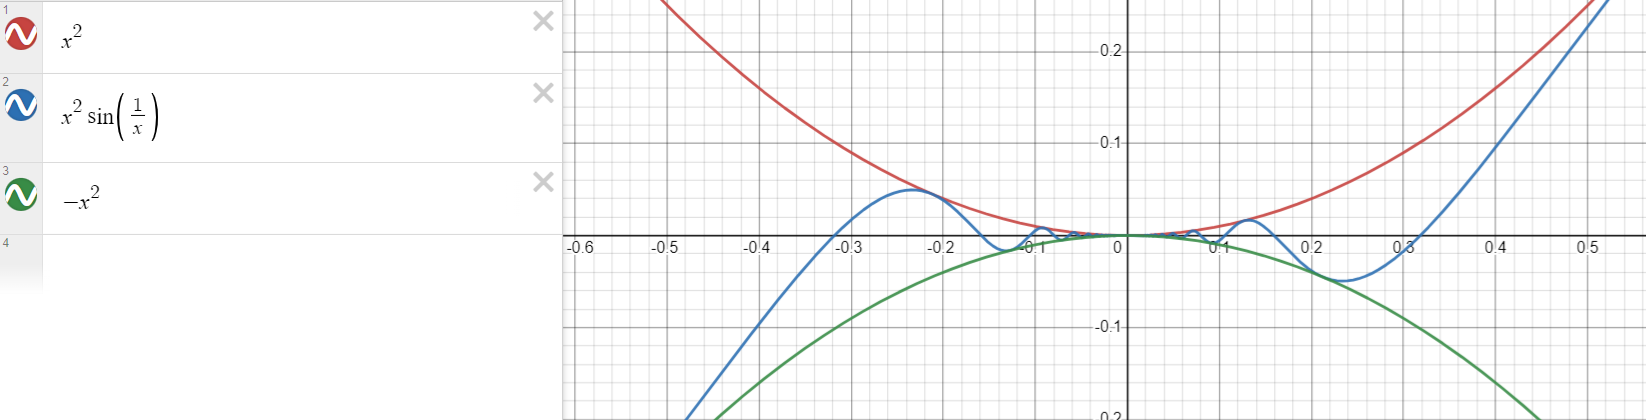
\includegraphics[width=0.99\linewidth]{tasks/task10/image.png}
\end{figure}
 
$f$ дифференцируема по Фреше в $x \neq 0$ (по правилу Лейбница):
\[\begin{aligned}
& {(x + h)}^{2} = x^2 +2xh+ \bar{o}(|h|)\\
& \sin{\frac{1}{x+h}} = \sin{\frac{1}{x}} + \frac{-1}{x^2} \cos{\frac{1}{x}}h + \bar{o}(|h|)
\end{aligned}\]
$|f(x)| \leq x^2 \implies f^{\prime}(0)=0$ и $f(x)-f(0)=f(x) =\bar{o}(|x|), |x| \rightarrow 0 $
то есть f диф. по Фреше в 0, тогда и на всем $\mathbb{R}$

Предположим противное: $f$ строго дифференцируемо в $0$.

По определению,  для любого $\varepsilon>0$ существует $\delta>0$ такое, что для любых $x_1, x_2 \in O_\delta\left(x_0\right)$ выполнено
\[\begin{aligned}
&|f\left(x_1\right)-f\left(x_2\right)-A\left(x_1-x_2\right)|\leq \varepsilon|x_1-x_2| \\
&f^{\prime}(0)=0 \implies |f\left(x_1\right)-f\left(x_2\right)|\leq \varepsilon|x_1-x_2|\leq 2\varepsilon \delta \\
& x\neq 0:  f^{\prime}(x)=2 x \sin \frac{1}{x}+x^2 \cos \frac{1}{x}\left(-1 \cdot \frac{1}{x^2}\right)=2 x \sin \left(\frac{1}{x}\right)-\cos \frac{1}{x} \nrightarrow 0, x \rightarrow 0 \\
& \text{потому что } \lim _{x \rightarrow 0} x \sin \frac{1}{x}=0 \text{ и } \lim _{x \rightarrow 0} \cos \frac{1}{x} \text{ не существует.} \\
& \text{Тогда }\exists \xi_n \rightarrow 0 \quad\left|f^{\prime}\left(\xi_n\right)\right| \geqslant c>0 \\
& f\left(\xi_n+h_n\right)-f\left(\xi_n\right)=f^{\prime}\left(\xi_n\right) h_n+\bar{o}\left(h_n\right) \text{ (по опр. диф. по Фреше)}\\
& h_n \longrightarrow 0 :\\
& \left|f\left(\xi_n+h_n\right)-f\left(\xi_n\right)\right| \geqslant C\left|h_n\right|
\end{aligned}\]
Получили противоречие. $f$ не является строго дифференцируемой в нуле.
\end{task}

\begin{task}
Привести пример функции $f: \mathbb{R} \rightarrow \mathbb{R}$, всюду дифференцируемой по Фреше, но не строго дифференцируемой в нуле.

\textbf{Доказательство:}
Рассмотрим функцию $f$:
\[
f(x)= \begin{cases}0, & x=0 \\ x^2 \sin \left(\frac{1}{x}\right), & x \neq 0\end{cases} 
\]

\begin{figure}[h!]
\centering
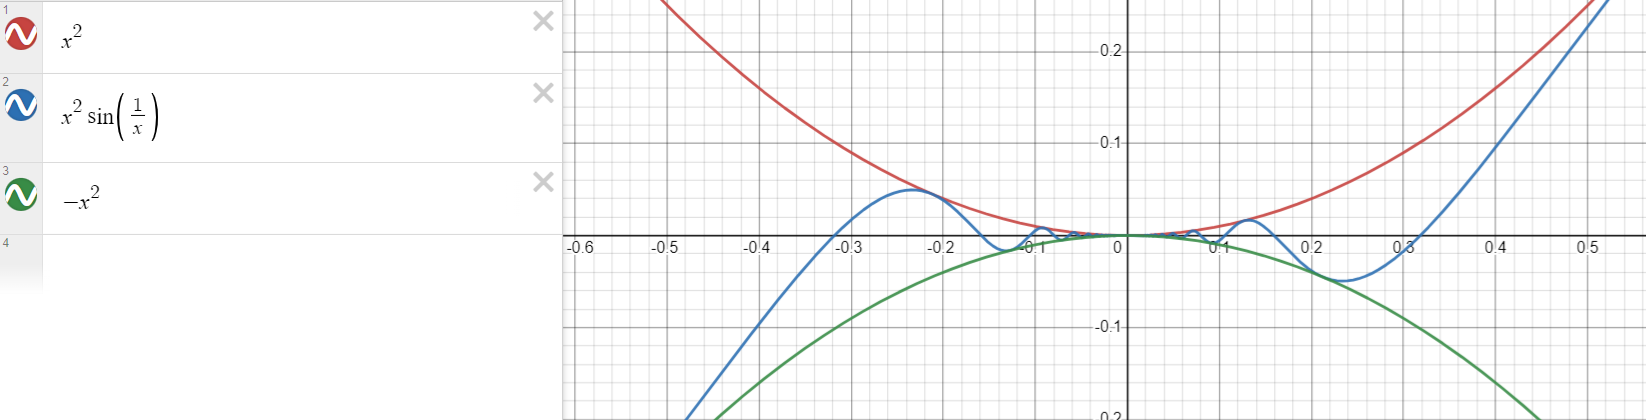
\includegraphics[width=0.99\linewidth]{tasks/task10/image.png}
\end{figure}
 
$f$ дифференцируема по Фреше в $x \neq 0$ (по правилу Лейбница):
\[\begin{aligned}
& {(x + h)}^{2} = x^2 +2xh+ \bar{o}(|h|)\\
& \sin{\frac{1}{x+h}} = \sin{\frac{1}{x}} + \frac{-1}{x^2} \cos{\frac{1}{x}}h + \bar{o}(|h|)
\end{aligned}\]
$|f(x)| \leq x^2 \implies f^{\prime}(0)=0$ и $f(x)-f(0)=f(x) =\bar{o}(|x|), |x| \rightarrow 0 $
то есть f диф. по Фреше в 0, тогда и на всем $\mathbb{R}$

Предположим противное: $f$ строго дифференцируемо в $0$.

По определению,  для любого $\varepsilon>0$ существует $\delta>0$ такое, что для любых $x_1, x_2 \in O_\delta\left(x_0\right)$ выполнено
\[\begin{aligned}
&|f\left(x_1\right)-f\left(x_2\right)-A\left(x_1-x_2\right)|\leq \varepsilon|x_1-x_2| \\
&f^{\prime}(0)=0 \implies |f\left(x_1\right)-f\left(x_2\right)|\leq \varepsilon|x_1-x_2|\leq 2\varepsilon \delta \\
& x\neq 0:  f^{\prime}(x)=2 x \sin \frac{1}{x}+x^2 \cos \frac{1}{x}\left(-1 \cdot \frac{1}{x^2}\right)=2 x \sin \left(\frac{1}{x}\right)-\cos \frac{1}{x} \nrightarrow 0, x \rightarrow 0 \\
& \text{потому что } \lim _{x \rightarrow 0} x \sin \frac{1}{x}=0 \text{ и } \lim _{x \rightarrow 0} \cos \frac{1}{x} \text{ не существует.} \\
& \text{Тогда }\exists \xi_n \rightarrow 0 \quad\left|f^{\prime}\left(\xi_n\right)\right| \geqslant c>0 \\
& f\left(\xi_n+h_n\right)-f\left(\xi_n\right)=f^{\prime}\left(\xi_n\right) h_n+\bar{o}\left(h_n\right) \text{ (по опр. диф. по Фреше)}\\
& h_n \longrightarrow 0 :\\
& \left|f\left(\xi_n+h_n\right)-f\left(\xi_n\right)\right| \geqslant C\left|h_n\right|
\end{aligned}\]
Получили противоречие. $f$ не является строго дифференцируемой в нуле.
\end{task}

\begin{task}
Привести пример функции $f: \mathbb{R} \rightarrow \mathbb{R}$, всюду дифференцируемой по Фреше, но не строго дифференцируемой в нуле.

\textbf{Доказательство:}
Рассмотрим функцию $f$:
\[
f(x)= \begin{cases}0, & x=0 \\ x^2 \sin \left(\frac{1}{x}\right), & x \neq 0\end{cases} 
\]

\begin{figure}[h!]
\centering
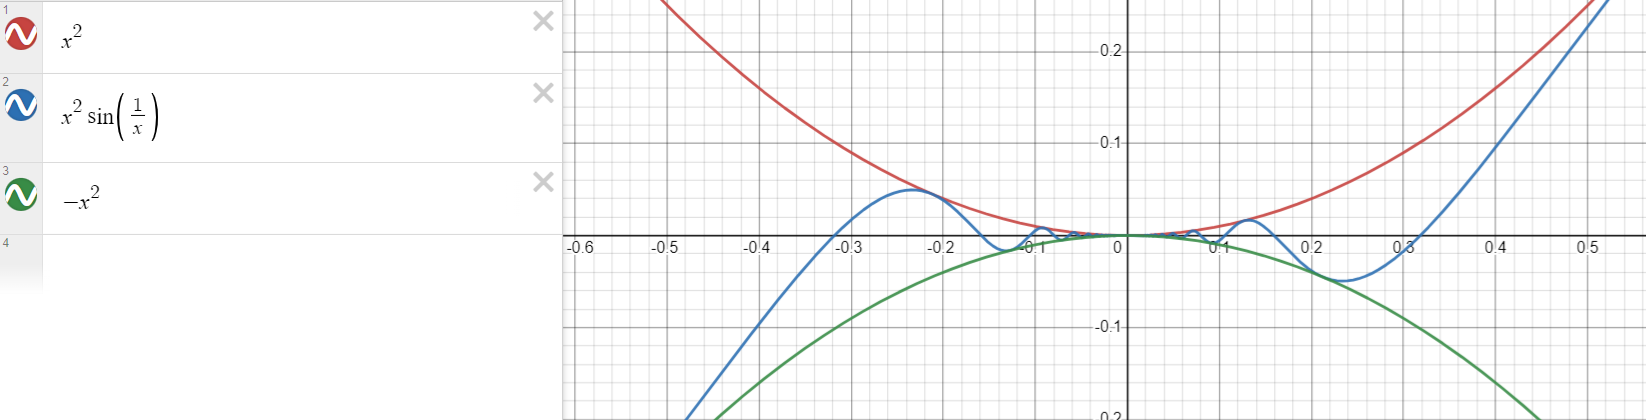
\includegraphics[width=0.99\linewidth]{tasks/task10/image.png}
\end{figure}
 
$f$ дифференцируема по Фреше в $x \neq 0$ (по правилу Лейбница):
\[\begin{aligned}
& {(x + h)}^{2} = x^2 +2xh+ \bar{o}(|h|)\\
& \sin{\frac{1}{x+h}} = \sin{\frac{1}{x}} + \frac{-1}{x^2} \cos{\frac{1}{x}}h + \bar{o}(|h|)
\end{aligned}\]
$|f(x)| \leq x^2 \implies f^{\prime}(0)=0$ и $f(x)-f(0)=f(x) =\bar{o}(|x|), |x| \rightarrow 0 $
то есть f диф. по Фреше в 0, тогда и на всем $\mathbb{R}$

Предположим противное: $f$ строго дифференцируемо в $0$.

По определению,  для любого $\varepsilon>0$ существует $\delta>0$ такое, что для любых $x_1, x_2 \in O_\delta\left(x_0\right)$ выполнено
\[\begin{aligned}
&|f\left(x_1\right)-f\left(x_2\right)-A\left(x_1-x_2\right)|\leq \varepsilon|x_1-x_2| \\
&f^{\prime}(0)=0 \implies |f\left(x_1\right)-f\left(x_2\right)|\leq \varepsilon|x_1-x_2|\leq 2\varepsilon \delta \\
& x\neq 0:  f^{\prime}(x)=2 x \sin \frac{1}{x}+x^2 \cos \frac{1}{x}\left(-1 \cdot \frac{1}{x^2}\right)=2 x \sin \left(\frac{1}{x}\right)-\cos \frac{1}{x} \nrightarrow 0, x \rightarrow 0 \\
& \text{потому что } \lim _{x \rightarrow 0} x \sin \frac{1}{x}=0 \text{ и } \lim _{x \rightarrow 0} \cos \frac{1}{x} \text{ не существует.} \\
& \text{Тогда }\exists \xi_n \rightarrow 0 \quad\left|f^{\prime}\left(\xi_n\right)\right| \geqslant c>0 \\
& f\left(\xi_n+h_n\right)-f\left(\xi_n\right)=f^{\prime}\left(\xi_n\right) h_n+\bar{o}\left(h_n\right) \text{ (по опр. диф. по Фреше)}\\
& h_n \longrightarrow 0 :\\
& \left|f\left(\xi_n+h_n\right)-f\left(\xi_n\right)\right| \geqslant C\left|h_n\right|
\end{aligned}\]
Получили противоречие. $f$ не является строго дифференцируемой в нуле.
\end{task}

\begin{task}
    Рассмотрим задачу
    \begin{equation*}
        \int_{-T_0}^{T_0} x \sqrt{\dot{x}^2+1} d t \rightarrow \min , 
        x\left(T_0\right) = x \left( -T_0 \right) = \xi.
    \end{equation*}
    \begin{enumerate}
        \item Выписать уравнение Якоби, подобрать одно из его решений, 
        затем найти общее решение. 
        \item Пусть допустимых экстремалей две. Доказать, что одна из них 
        является точкой сильного минимума, а вторая не является точкой слабого минимума.
    \end{enumerate}


    \textbf{Peшение.} 
    \begin{definition}
        Говорят, что выполнено усиленное условие Лежандра, 
        если $\widehat L_{\dot{x}\dot{x}} > 0 \; \forall t \in [t_0, t_1]$.
    \end{definition}

    \begin{definition} Говорят, что выполнено условие Якоби, 
        если справедливо усиленное условие Лежандра, а решение уравнения Якоби
        \begin{equation*}
            -\frac{d}{d t}\left(\widehat{L}_{\dot{x} \dot{x}}(t) \dot{h}
                +\widehat{L}_{\dot{x} x}(t) h\right)
                +\left(\widehat{L}_{\dot{x} x}(t) \dot{h}
                +\widehat{f}_{x x}(t) h\right)=0 \quad 
                \Leftrightarrow \quad \frac{d}{d t}\left(\widehat{L}_{\dot{x} \dot{x}}(t) \dot{h}\right)
                =\left(\widehat{L}_{x x}(t)-\frac{d}{d t} \widehat{L}_{\dot{x} x}(t)\right) h
        \end{equation*}
        не обращается в ноль на интервале $\left(t_0, t_1\right)$ при начальных условиях: 
        $h\left(t_0\right)=0, \quad \dot{h}\left(t_0\right)=1$.
\end{definition}

1. Уравнение Якоби в данном случае имеет вид:
\begin{equation*}
    \ddot{h}-\frac{2}{C} \th (\frac{t}{C}) \dot{h}+\frac{1}{C^2} h = 0    
\end{equation*}
Оно имеет два линейно независимых решения: 
$h_1(t)=\operatorname{sh} \frac{t}{C}$ и $h_2(t)=\operatorname{ch} \frac{t}{C}-\frac{t}{C} \operatorname{sh} \frac{t}{C}$. 
Общее решение, подчиненное условию $h(-1)=0$, таково:

\begin{equation*}
h(t)=\left(\operatorname{ch} \frac{t}{C}-\frac{t}{C} \operatorname{sh} \frac{t}{C}\right) \operatorname{sh} \frac{1}{C}+\left(\operatorname{ch} \frac{1}{C}-\frac{1}{C} \operatorname{sh} \frac{1}{C}\right) \operatorname{sh} \frac{t}{C} .
\end{equation*}

2. Было показано (см. \ref{task6}), что экстремали существуют, 
если и только если $\xi \geq \xi_{*}=\operatorname{sh} \frac{1}{C_0}$, 
где $C_0=\operatorname{th} \frac{1}{C_0} \approx 1.5088 \ldots$ При этом, экстремаль задается формулой 
$x(t)=C \operatorname{ch} \frac{t}{C}$, а параметр $C>0$ есть корень уравнения $\varphi(C) = \xi$, 
где $\varphi(C) \stackrel{\text { def }}{=} C \operatorname{ch} \frac{1}{C}$. 

Функция $C \mapsto \varphi(C)$ выпукла, т.к. $\varphi^{\prime \prime}(C)=C^{-3} \operatorname{ch} \frac{1}{C}$. 
Ее минимум достигается в точке $C_0$, где $\varphi^{\prime}\left(C_0\right)=0$. Отметим, что
$$
\varphi^{\prime}(C)=\left[\operatorname{ch} \frac{1}{C}-\frac{1}{C} \operatorname{sh} \frac{1}{C}\right]
$$

Если $\xi > \xi_{*}$, то существуют ровно два значения $C_1 \in\left(0, C_0\right)$ и $C_2>C_0$, 
которые удовлетворяют условию $\varphi(C)=R$. Покажем, что экстремаль $\widehat{x}_2=C_2 \operatorname{ch} \frac{1}{C_2}$ 
доставляет сильный (локальный) минимум, а экстремаль $\widehat{x}_1=C_1 \operatorname{ch} \frac{1}{C_1}$ 
не является ни слабым минимумом, ни слабым максимумом. Прежде всего, отметим, что для обеих экстремалей выполнено 
усиленное условие Лежандра, а именно: $\widehat{f}_{\dot{x} \dot{x}}(t)=C \mathrm{ch}^{-2} \frac{t}{C} > 0$ 
и потому ни одна из них не является локальным максимумом. \par


Так как $h(0)=\operatorname{sh} \frac{1}{C} \neq 0$, то нули функции $h$ совпадают с нулями функции
$$
z: t \mapsto z(t)=\frac{h(t)}{\operatorname{sh} \frac{1}{C} \operatorname{sh} \frac{t}{C}}=\left(\operatorname{cth} \frac{t}{C}-\frac{t}{C}\right)+\left(\operatorname{cth} \frac{1}{C}-\frac{1}{C}\right)
$$

Заметим, что $z^{\prime}(t)<0$, а $z(1) = \frac{2 \varphi^{\prime}(C)}{\operatorname{sh} \frac{1}{C}}$. 
Поэтому, если $z(1)<0 \Leftrightarrow C=C_1$, то условие Якоби не выполнено, а если $z(1) > 0 \Leftrightarrow C=C_2$, 
то выполнено усиленное условие Якоби.

\end{task}

\end{document}
